\section{Introduction}
As this thesis is primarily an exploration of epitaxial interfaces using a wide array of experimental techniques, the background material here will cover the theoretical concepts that are regularly drawn upon to present the growth models presented elsewhere.
Models presented later in the document are primarily of a conceptual nature and as such background here will also be presented in that manner.
Mathematics will be used where applicable but will be generally avoided, as the restricted assumptions are of little use to the work presented later.

There are a few key theoretical concepts which must be understood to best describe the expanded epitaxial model proposed here.
The first, and most integral to the discussion is an examination of the model of epitaxy as now defined in the literature.
This is integral to differentiate where the material systems examined diverge from the idealized models presented in the literature.
As part of the examination of epitaxy, particular attention will be given to nucleation and clusters on surfaces as this examination hinges on the role of the epitaxial interface.
Beyond epitaxy, the other key subjects which require background exposition are surface reconstructions, which describe the properties of the other side of the epitaxial interface, the substrate, and atomic bonding, the connections which reach across the epitaxial interface.

\section{Epitaxy}
\subsection{Homoepitaxy --- Separating Thermodynamics from Kinetics} The most basic form of epitaxy that can be conceived of is homoepitaxy, that is, where a material \textbf{A}, is grown on an existing single crystal of that same material \textbf{A}.
In this growth process, the crystal structure, lattice constants and chemistry are identical across the epitaxial interface.
Despite this ideal situation, the growth of perfect homoepitaxial crystals is not guaranteed.
The fact that a homoepitaxial growth can be defective in a number of ways is due to the difference between the thermodynamics and kinetics of the epitaxial growth process.
Thermodynamically, one would expect that since the lowest energy state for the system would be the continuation of the existing single crystal via the homoepitaxial growth process, however, due to kinetics, the exact conditions of growth process can have a substantial impact on the outcome crystal.

The homoepitaxial growth process is an excellent model system to separate the role of thermodynamics in growth from that of the kinetics.
Kinetics in an epitaxial growth process refers to the role time plays in an epitaxial growth process, usually examined via rates.
There are two fundamental kinetic rate types involved in epitaxial growth, those which can be directly controlled by the experimenter and those which are primarily properties of the material system and can only be indirectly influenced by the experimenter, the most important kinetic processes in epitaxy are shown as \cref{fig:back_epi_rates}.
\begin{figure}
 \centering 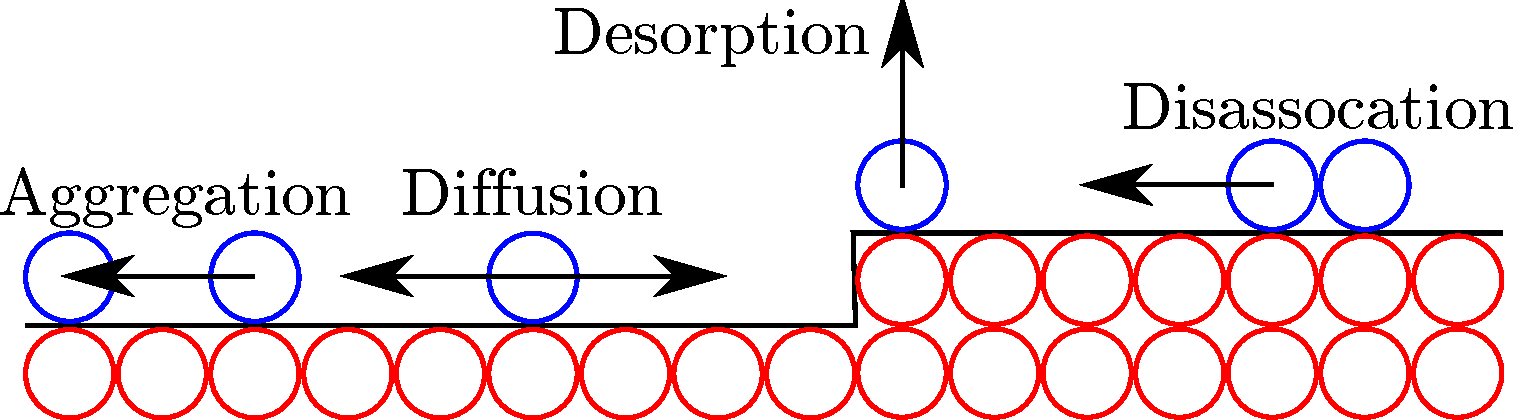
\includegraphics[width=0.9\textwidth]{back_epi_rates}
 \caption[Kinetic Processes of atoms on surfaces]{\label{fig:back_epi_rates}Kinetic processes with Arrhenius rates which participate during epitaxy}
\end{figure}

The most common experimentally controlled rates in an epitaxial growth are the rate of addition of atoms to the growth interface, and the temperature and the rate the temperature is increased or decreased during a growth.
The rate of atom addition, or the growth rate is a key parameter and in homoepitaxial growth, can reveal the role kinetics plays in growth.
If the rate at which atoms are added to an epitaxial interface is extremely high, the atoms will have no time to move towards their thermodynamically preferred location.
The resulting material that grows will consist of the layers of atoms stacked randomly where they first hit the substrate and were immediately covered by more atoms.
Such a configuration is not an epitaxial growth, rather the film is likely to be amorphous or fine grained polycrystalline, yet there are no material limitations per-se that are causing the poor growth, it is purely kinetic.
As the growth rate is lowered adatoms are allowed more time to move via diffusion, they may register in some regions, but not in others, resulting in a partially crystalline growth.
As the deposition rate is further reduced, depending upon the material, the film may grow in a fully crystalline nature, but be twinned or contain stacking faults.
The bonding along \{111\} directions in a zincblende crystal is susceptible to faults due to their relative rotational symmetry, the exact susceptibility is known by the Stacking Fault Energy (SFE)\cite{Duffar2010}.
Stacking fault energies in semiconductor materials vary from as low as single digit mJ/m\textsuperscript{2} (CdTe 9~mJ/m\textsuperscript{2}), to over 200 mJ/m\textsuperscript{2} (C 285~mJ/m\textsuperscript{2})\cite{Takeuchi1999}.
This energy is a measure of the cost of making such a defect in a crystal, so crystals with low SFE are very susceptible to twinning during growth.
At yet lower growth rates the adatoms have time to find their low energy states with respect to twins, finally arriving at a single crystal.
\begin{align}
 A = A_0 e^{-\frac{E_0}{kT}} \label{eqn:arrhenius} \\
 A = - v a^2 e^{-\frac{E_0}{kT}}
\end{align}
While the directly controlled deposition rate seems to be severely limited by defect formation and stacking of adatoms, there are large number of kinetic processes during growth that can be indirectly influenced by an experimenter through the control of temperature.
Fundamentally, the other kinetic processes fundamental to growth are all of the Arrhenius type, as shown in \cref{eqn:arrhenius}.
A process which is exponential, with a pre-factor (\textbf{A\textsubscript{0}}) and an activation energy (\textbf{E\textsubscript{0}}).
For crystalline surfaces, the pre-factor can be further defined as an attempt frequency or attempt rate (\textbf{v}) and the surface lattice spacing (\textbf{a})\cite{Einax2013}.
As such, these processes have an exponential dependence on the temperature at which growth occurs.
Among the other kinetic processes involved in growth, the most important are surface diffusion, bulk diffusion, desorption and aggregation/disassociation.
Through the increase in temperature the rates of all of these (except nucleation) processes increases.
This has a strong impact on the epitaxial process.

The key kinetic factor to the improvement of epitaxial growth is the increase in the surface diffusion rate.
Surface diffusion of adatoms during growth is the process by which a newly adsorbed atom from the impinging atoms finds its lowest energy position on the epitaxial surface.
Increases in temperature increase the rate at which these adatoms move, increasing the probability that they will find their lowest energy position before they are encapsulated by additional atoms.
While increases in temperature will improve the mobility of adatoms, increases in temperature also increase other processes.
Bulk diffusion is the process by which adatoms at the epitaxial interface diffuse into the substrate through exchange with other atoms or travel interstitially.
In homoepitaxy this process is irrelevant, but in any chemically dissimilar growth such a process distorts the interface, which is generally not preferred.
Furthermore, as temperature increases, adatoms can begin to desorb, leaving the epitaxial interface, slowing growth and under extreme circumstances, the substrate itself can also begin to lose atoms.
Finally, at very high surface diffusion rates, adatoms may not ever attach to others, preventing nucleation of new layers of crystal.

The kinetics of growth are thus balanced between the intended growth rate, determined by the delivery of atoms to the epitaxial interface, and a temperature that is high enough to ensure single crystal growth, but not too high to cause breakdown of the epitaxial process, a delicate balance.

\subsection{Heteroepitaxy} Heteroepitaxy covers a wide range of \textbf{A} on \textbf{B} epitaxy systems, as such, the following treatment will start from the basics established in homoepitaxy and gradually add the levels of complexity found in real-world systems and consider how they add to the model.

\subsubsection{Strained Heteroepitaxy} The first step in the complication from homoepitaxy to heteroepitaxy is to introduce a difference in the lattice constants between the substrate and the growing epitaxial crystal, while maintaining the crystal structures and chemical composition.
When there is a strong chemical bond between the two crystals across the interface, both feel a distortion from their ideal crystal structures, one is compressed slightly, while the other is tensioned\cite{Dunstan1997}.
Nature has provided an ideal model system which perfectly fits these requirements, the Si\(_{1-x}\)Ge\(_x\) system grown on silicon\cite{Paul2004}.
In Si\(_{1-x}\)Ge\(_x\), germanium substitutes into the silicon lattice randomly, maintaining the same valence and diamond structure.
The lattice constant varies nearly linearly between silicon and germanium as in \cref{eqn:sige}.
\begin{equation}
 a_{Si_{1-x}Ge_x} = 0.5431 + 0.01992x + 0.0002733x^2 \label{eqn:sige}
\end{equation}

The difference between lattice constants is expressed as the lattice mismatch as in \cref{eqn:mismatch}.
Negative values indicate that the growing layer is strained in tension by bonding to the substrate, while positive values indicate that growing layer is strained in compression by bonding to the substrate.
The fundamental physical parameter describing such mismatched system is strain, that is, the distortion of atoms from the thermodynamic equilibrium positions, due to bonding to a mismatched substrate.
Strain can be conceptualized as energy stored within the stretched bonds of the epitaxial layer, like a spring displaced from its equilibrium position, increasing the internal energy within the epitaxial crystal.
\begin{figure}
 \centering 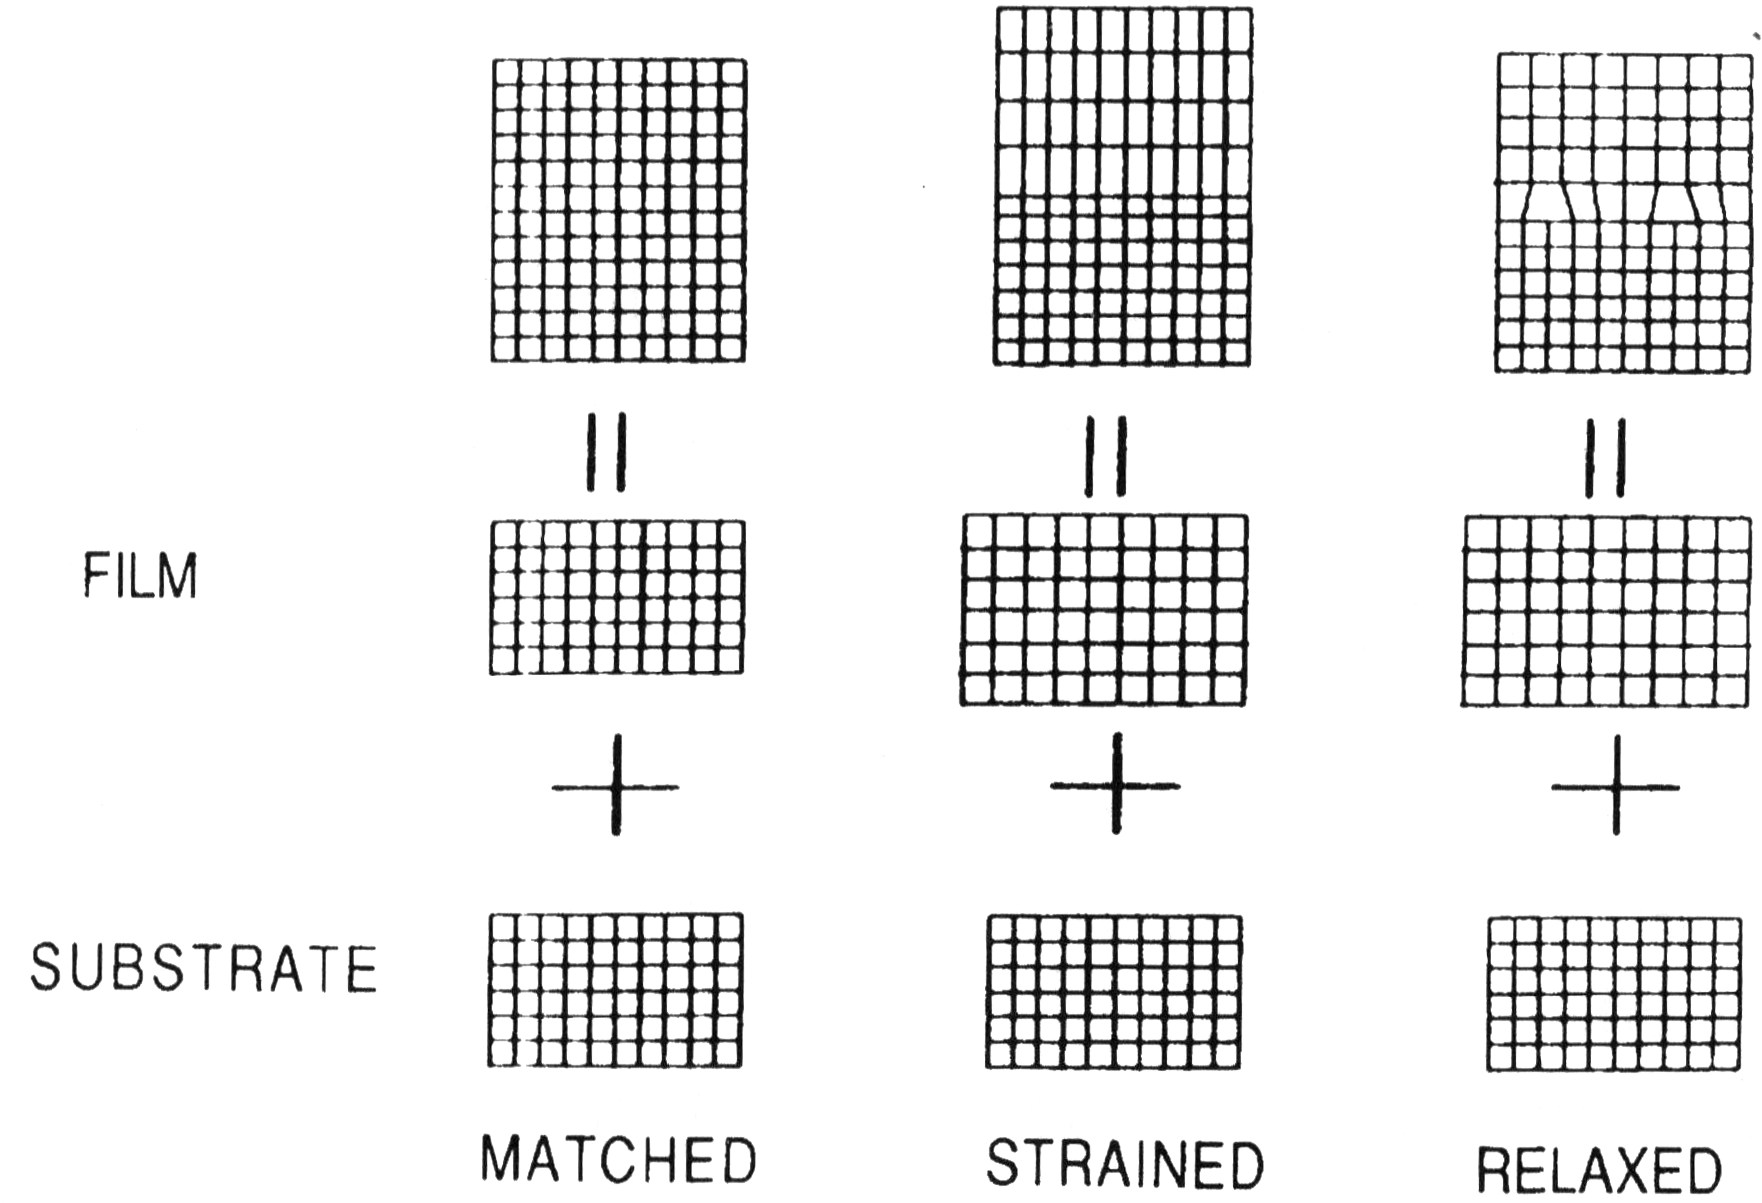
\includegraphics[width=0.8\textwidth]{back_strain}
 \caption[Unit cell strain visualization]{\label{fig:back_strain}Effects of strain on unit cell of epitaxial crystal a) matched, no strain b) strained, but pseudomorphic, lattice is only distorted c) highly strained resulting in dislocations to relax strain\cite{ohring2001materials} (used with permission)}
\end{figure}

Through the examination of the Si\(_{1-x}\)Ge\(_x\) system grown on silicon, the effect of pure compressive strain on an epitaxial process has been examined.
As an epitaxial crystal of Si\(_{1-x}\)Ge\(_x\) is grown on a silicon substrate, the strain energy in the crystal increases with thickness.
The growing epitaxial crystal maintains the lateral lattice constant of the substrate, and conserves it's volume by changing it's vertical lattice constant, this is known as pseudomorphic growth.
Beyond a certain point, the energy required to add another layer of strained crystal is too much, and the strain is relieved through the introduction of a defects in the form of dislocations.
In a dislocation, the bonding between the epitaxial crystal and the substrate is broken to allow the crystal to expand, leaving a dangling bond at the substrate.
Such a process is random so defects are located randomly at the interface.
The exact thickness where a pseudomorphic growth will introduce defects in order to relieve strain is known as the critical thickness and is dependent upon several factors.
These factors include the strength of the bonds across the epitaxial interface, the bond strength within the epitaxial layer, and the energetic cost of forming a dislocation in terms of atomic movement and dangling bonds.
These last two factors are impacted by kinetics as there is often a large activation energy associated with defect formation.
\Cref{fig:back_strain_regions} shows the experimental curve for the model system Si\(_{1-x}\)Ge\(_x\) grown on Si including the dividing line between pseudomorphic and dislocated growth due to strain.
The critical thickness model is qualitatively similar for other systems that have similar growth properties.
\begin{equation}
 f = \frac{a_f - a_s}{a_s} \label{eqn:mismatch}
\end{equation}
\begin{figure}
 \centering 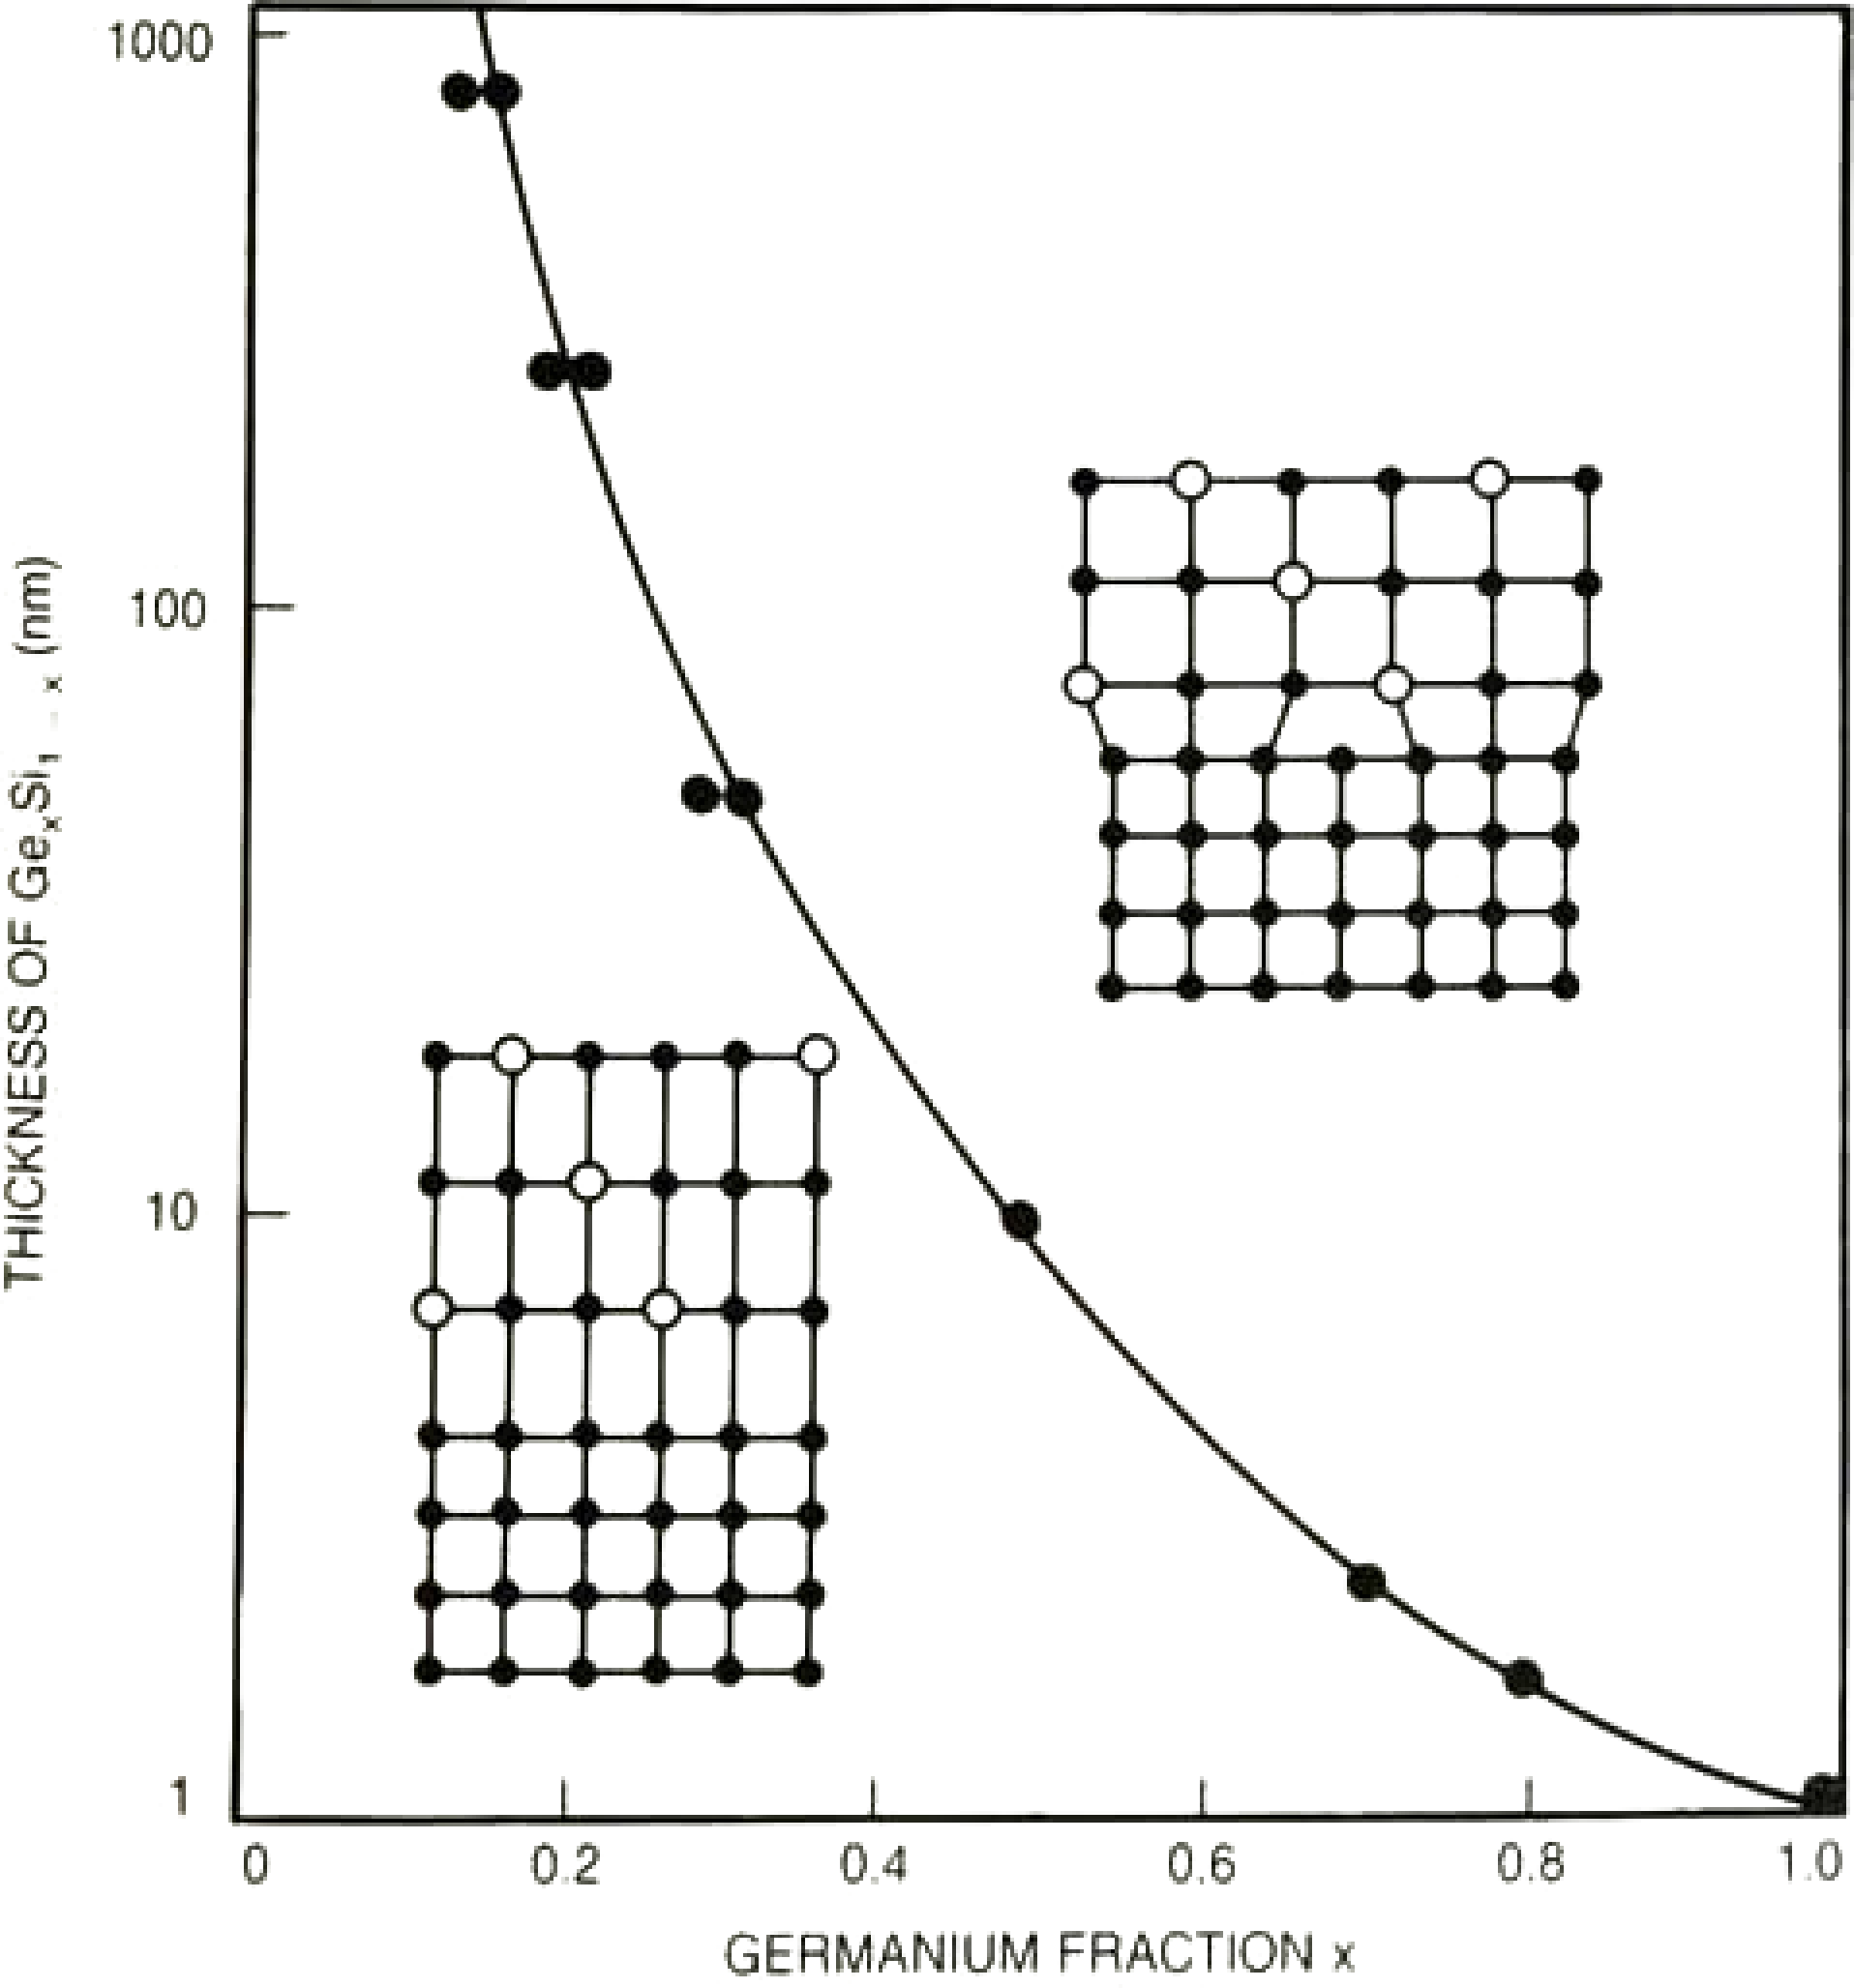
\includegraphics[width=0.6\textwidth]{back_strain_regions}
 \caption[Critical thickness dependence on strain]{\label{fig:back_strain_regions}Critical thickness versus germanium fraction of Si\(_{1-x}\)Ge\(_x\), showing regions of pseudomorphic growth and relaxed growth by dislocations (Reprinted with permission from Bean \textit{et al.}\cite{Bean1986}.
  Copyright 1986, American Institute of Physics.)}
\end{figure}
\subsubsection{Chemically Dissimilar Heteroepitaxy} On the other side of the heteroepitaxy spectrum are those epitaxial growths that have commensurate crystal structures but differ in their chemical compositions.
There few material systems which provide an ideal model for a lattice matched (zero strain), but chemically dissimilar epitaxial growth.
The most well characterized model system available is a lattice matched III-V semiconductor on germanium, specifically GaAs, which has a small (\(<\)0.1\%) lattice mismatch.
GaAs is a binary semiconductor with the zincblende crystal structure, which is a cubic crystal identical to silicon and germanium's diamond structure, but with a two-atom basis (Ga, As).
The crystal is covalently bonded as with Si, but has a \(\sim\)30\% ionic character due to differences in electronegativity\cite{Christensen1987}.

The zincblende crystal structure is due to two atoms of different valence (group III-group V), which forms a polar crystal structure, with the group-III atom supplying three electrons and the group-V atom supplying five electrons to the bonding structure.
The two-atom basis of zincblende breaks the diamond crystal structure such that the structure is no longer centrosymmetric, meaning that opposite directions in the crystal are no longer symmetrically equivalent.
This breaking of symmetry in the crystal means that the ordering of the group-III and group-V atoms at the epitaxial interface matters for crystal growth.
This problem is known as ``polar-on-nonpolar'' epitaxy\cite{Biegelsen1992,Kroemer1987}.
\begin{figure}
 \centering 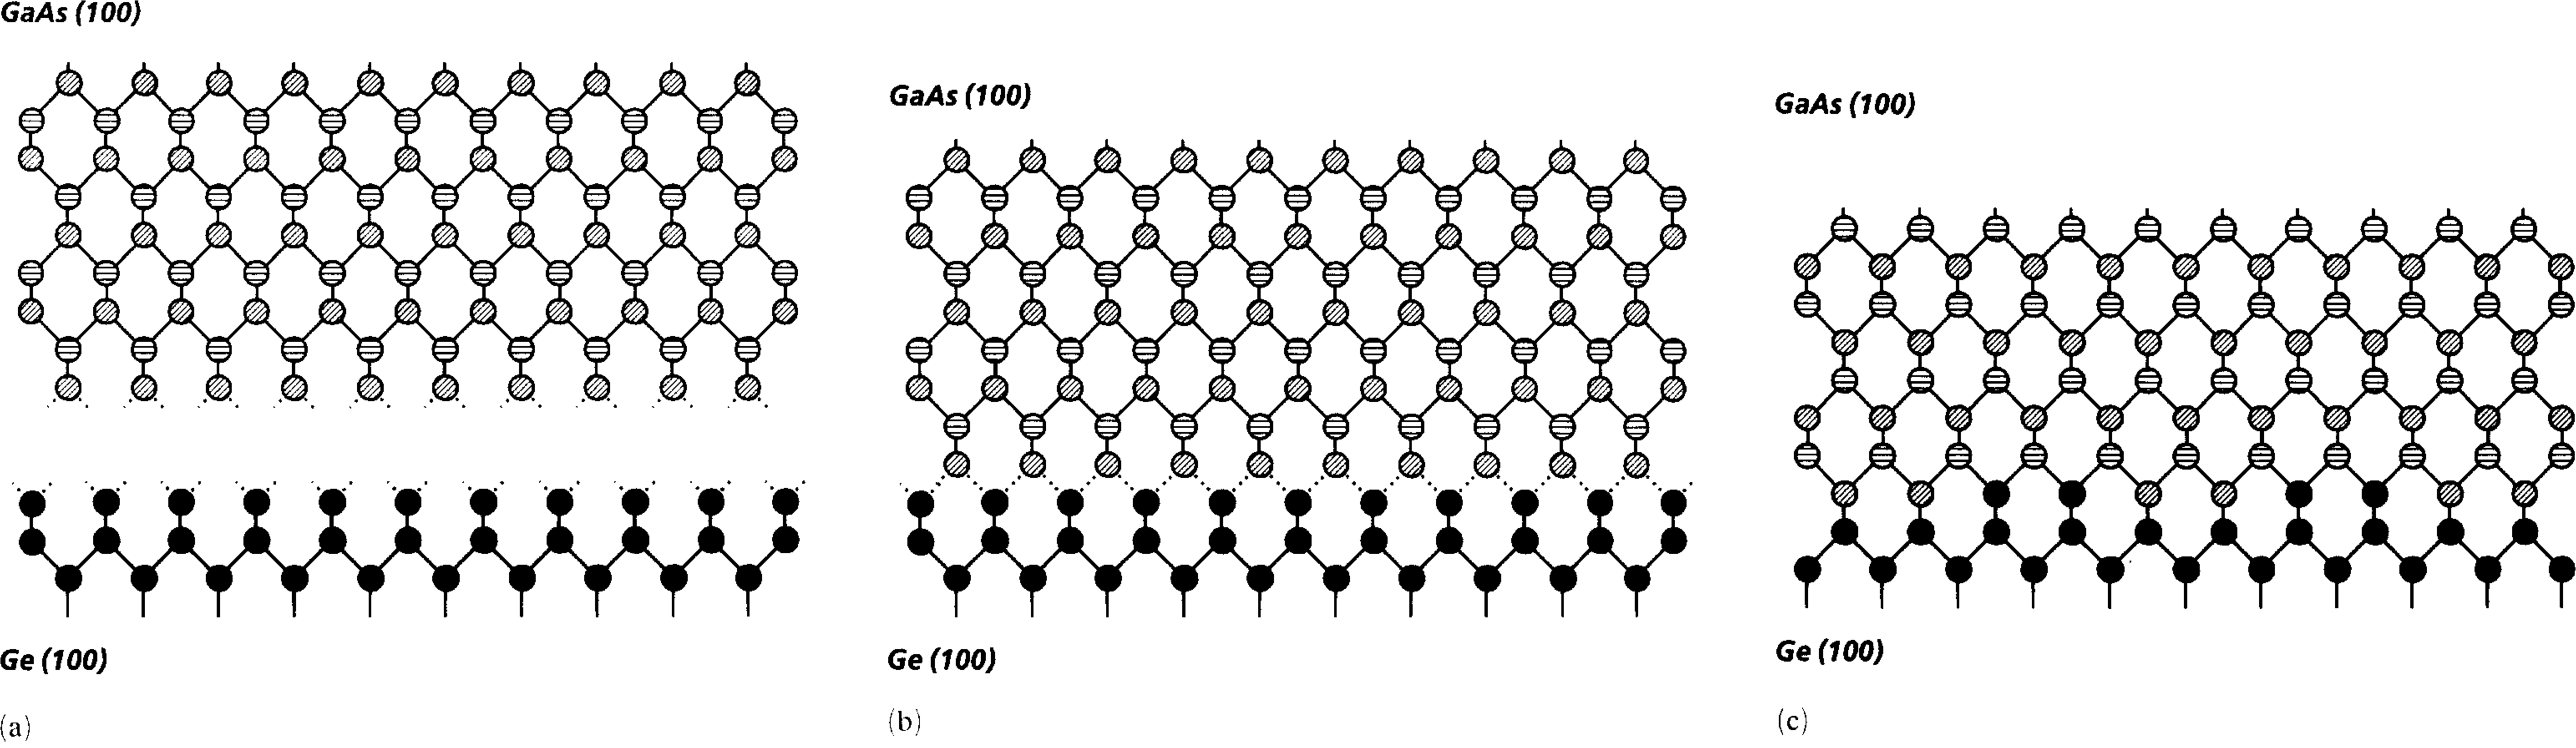
\includegraphics[width=\textwidth]{back_polar_model}
 \caption[Atomic model of polar on non-polar epitaxy]{\label{fig:back_polar_model}GaAs (polar) on Ge (non-polar) ideal epitaxy model a) separate crystals b) bonding showing surface charge c) atomic exchange resolving surface charge\cite{Biegelsen1992}(used with permission)}
\end{figure}

If the truncated crystal surface of such a polar semiconductor is brought towards the truncated surface of a silicon crystal as in \cref{fig:back_polar_model}, the interface that results, while all bonds will be satisfied with no strain, will not be satisfied electronically.
There will be a deficit (group-III) or excess (group-V) of electrons participating in bonding at the interface, leaving a layer of excess charge.
Such excess charge would be massive as it forms across the entire interface.
During growth of a crystal, rather than the thought experiment just discussed, we could expect that the surface charge would be a driving force for an atomic rearrangement at the interface as in \cref{fig:back_polar_model}c.
Experimental results have shown that several different rearrangements are possible.
The interface region can become three dimensional with the substrate and epitaxial layer atoms swapping to balance the number of excess and deficient bonds, resulting in an overall neutral charge.
Defects of different types can also form, resulting in dangling bonds which can compensate charge.
Some orientations of the crystal substrate, such as (211) offer unique lattice sites such that the charge neutrality is maintained automatically, which has motivated some of the work presented in \cref{sec:211}.

In addition to issues of charge neutrality at chemically dissimilar ideal epitaxial interfaces, there is a second issue.
This issue only arises in practical growth situations, because real substrates are never perfectly aligned with their intended crystal orientation.
These substrates, when offcut even the smallest amount from the intended orientation, will reconstruct into terraces of the primary crystal orientation separated by atomic height steps, the details of this process will be covered in \cref{sec:reconstruction}.
When those steps are single steps, that is, a/2 in height, adjacent terraces expose different sublattices of the diamond structure and these two sublattices have their exposed bonds rotated relative to each other.
When a crystal is grown atop such a substrate, the growth on adjacent crystals will also be offset by a/2.
While such an offset is not detrimental to the substrate itself, the zincblende crystal structure with two different atoms, when offset by the same amount, will result in a misalignment of the growing crystal at the step edges.
The step edge will contain III-III or V-V bonds, a section known as an anti-phase boundary, a defect that causes significant electrical defects and unintentional doping due to uncompensated bonds.
Sufficient care must be taken when preparing substrates (as noted later in \cref{sec:reconstruction}) to avoid these highly detrimental anti-phase boundaries.

\subsection{Clusters and Nucleation} As will be noted throughout this document, the key factor in the growth of epitaxial crystals is the properties of the epitaxial interface.
The two generalized properties that impact this interface are the energy and symmetry at the interface.
The initial stages of the epitaxial growth process is a key step which reveals the complex interplay of strain, energy and symmetry, through the form of the nucleation of the epitaxial crystal.

A key qualitative measure of the affinity of a given crystal to grow on another crystal is what is termed the nucleation mode of the epitaxial crystal.
Qualitatively, the nucleation mode of a given epitaxial crystal \textbf{A} on a substrate \textbf{B}, describes the affinity for the atoms in \textbf{A} to wet (spread out and contact) the substrate versus sticking to each other.
The wetting and dewetting of a given system is described by Young's equation, as in \cref{eqn:youngs}.
Young's equation describes the balance of three energies, the solid-liquid energy (\(\gamma_{SL}\)), the solid-gas energy (\(\gamma_{SG}\)) and the liquid-gas energy (\(\gamma_{LG}\)), through a parameter denoted the contact angle.
The contact angle is the key parameter which determines wetting characteristics of a system.
\begin{equation}
 \gamma_{SL} + \gamma_{LG} \cos{\theta_c} = \gamma_{SG} \label{eqn:youngs}
\end{equation}
Young's equation can be visualized as an isotropic droplet of the epitaxial crystal material sitting atop a substrate, making some contact angle with the substrate, as in \cref{fig:back_epi_young}a.
Contact angles of less than 90\degree{} are denoted as wetting a surface, while angles greater than 90\degree{} are denoted as dewetting a surface.
Young's equation assumes the wetting material is isotropic, that is, has no preferred direction or orientation.
Such a situation is common for polymers, liquids, and materials heated above their melting point.
For crystalline materials, there are preferred close packed surfaces which have lower energy.
The additional energy consideration, visualized in \cref{fig:back_epi_young}b shows how surface clusters form Wulff shapes, balancing surface interface energies and the energy of exposed crystal facets\cite{Venables1984}.
\begin{figure}
 \centering 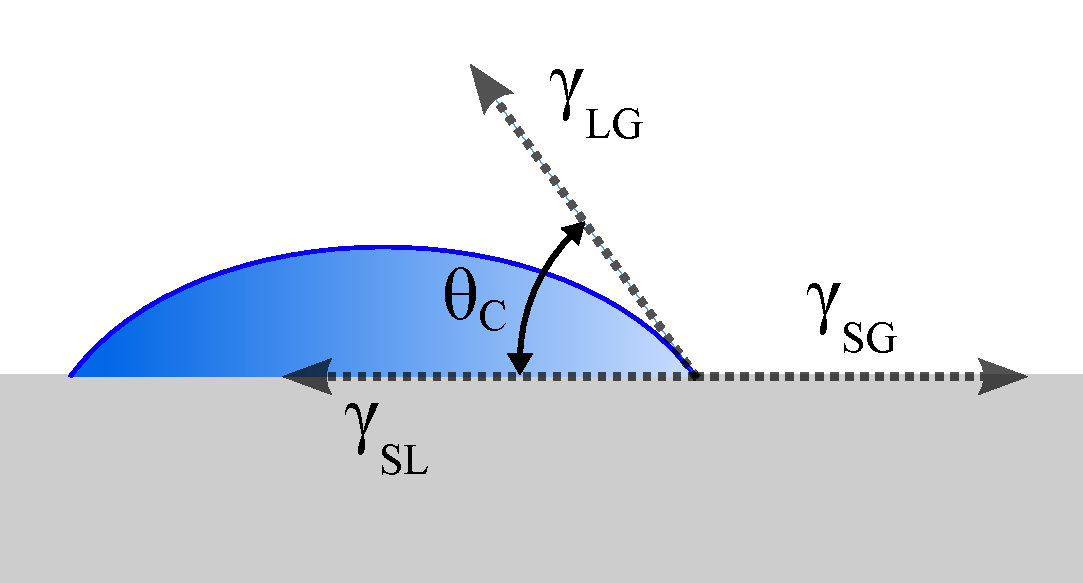
\includegraphics[width=0.9\textwidth]{back_epi_young}
 \caption[Young's equation]{\label{fig:back_epi_young}a) Young's equation visualized as an isotropic droplet sitting atop a substrate, with surface energies and contact angle labelled b) Minimum surface energy Wulff shape of a crystalline material atop a substrate, with surface energies, contact angle and crystal surface energy (after \cite{wikipedia_surface_energy})}
\end{figure}

Since Young's equation (and Wulff shapes) describe the preference of a given material to stick to a substrate or to itself, such wetting and dewetting can naturally be extended to describe the modes of growth when a film is deposited onto a substrate.
During epitaxial nucleation, incoming atomic material is incorporated into thin films as one of three modes, named island nucleation (Volmer–Weber), layer-by-layer nucleation (Frank–van der Merwe), and layer plus island (Stranski-Krastanov) or mixed-mode nucleation\cite{Venables1984}, as in \cref{fig:back_nucleation_regions}.
These modes describe the preference for the deposited atoms to spread out (wet) the growth interface or bunch up (dewet).

The energies in Young's equation are intrinsic to the crystal and chemical relationship between the epitaxial crystal and the substrate, as well as possibly the overlying gas.
Strain and chemical bonding are the two primary factors which influence the energy parameters which participate in the nucleation process.
The regions of have been mapped experimentally for several model systems, both chemically similar and strained, and the chemically dissimilar but unstrained, as shown in \cref{fig:back_nucleation_regions}.
Layer-by-layer nucleation and growth is most readily achieved when the epitaxial crystal and substrate are chemically compatible and have minimal strain\cite{Venables1984}.
For chemically incompatible systems nucleation is always island nucleation, as the epitaxial crystal would rather bond to itself than the substrate.
With increasing strain nucleation can begin as layer by layer, but transition to island after several layers.
Mixed mode growth is also common where the deposited atoms prefer to bond to the substrate much more strongly than to each other, resulting in an initial flat layer followed by island formation\cite{Venables1984}.
Nucleation modes also have a dependence on the rate of material deposition and the temperature of the substrate.
Systems which would prefer to form islands during nucleation can be restricted to layer-like growth modes by increasing the deposition rate or reducing the temperature.

For a generalized epitaxial system, there are other factors not considered as part of this simple model.
These nucleation modes do not consider the kinetics of the growth process, if atoms are delivered too quickly nucleation can form islands regardless of the predictions of Young's equation.
The conditions for optimal nucleation may be different than those of growth, especially in the case of mixed-mode, where changes in growth parameters during growth may lead to better outcomes overall.
\begin{figure}
 \centering 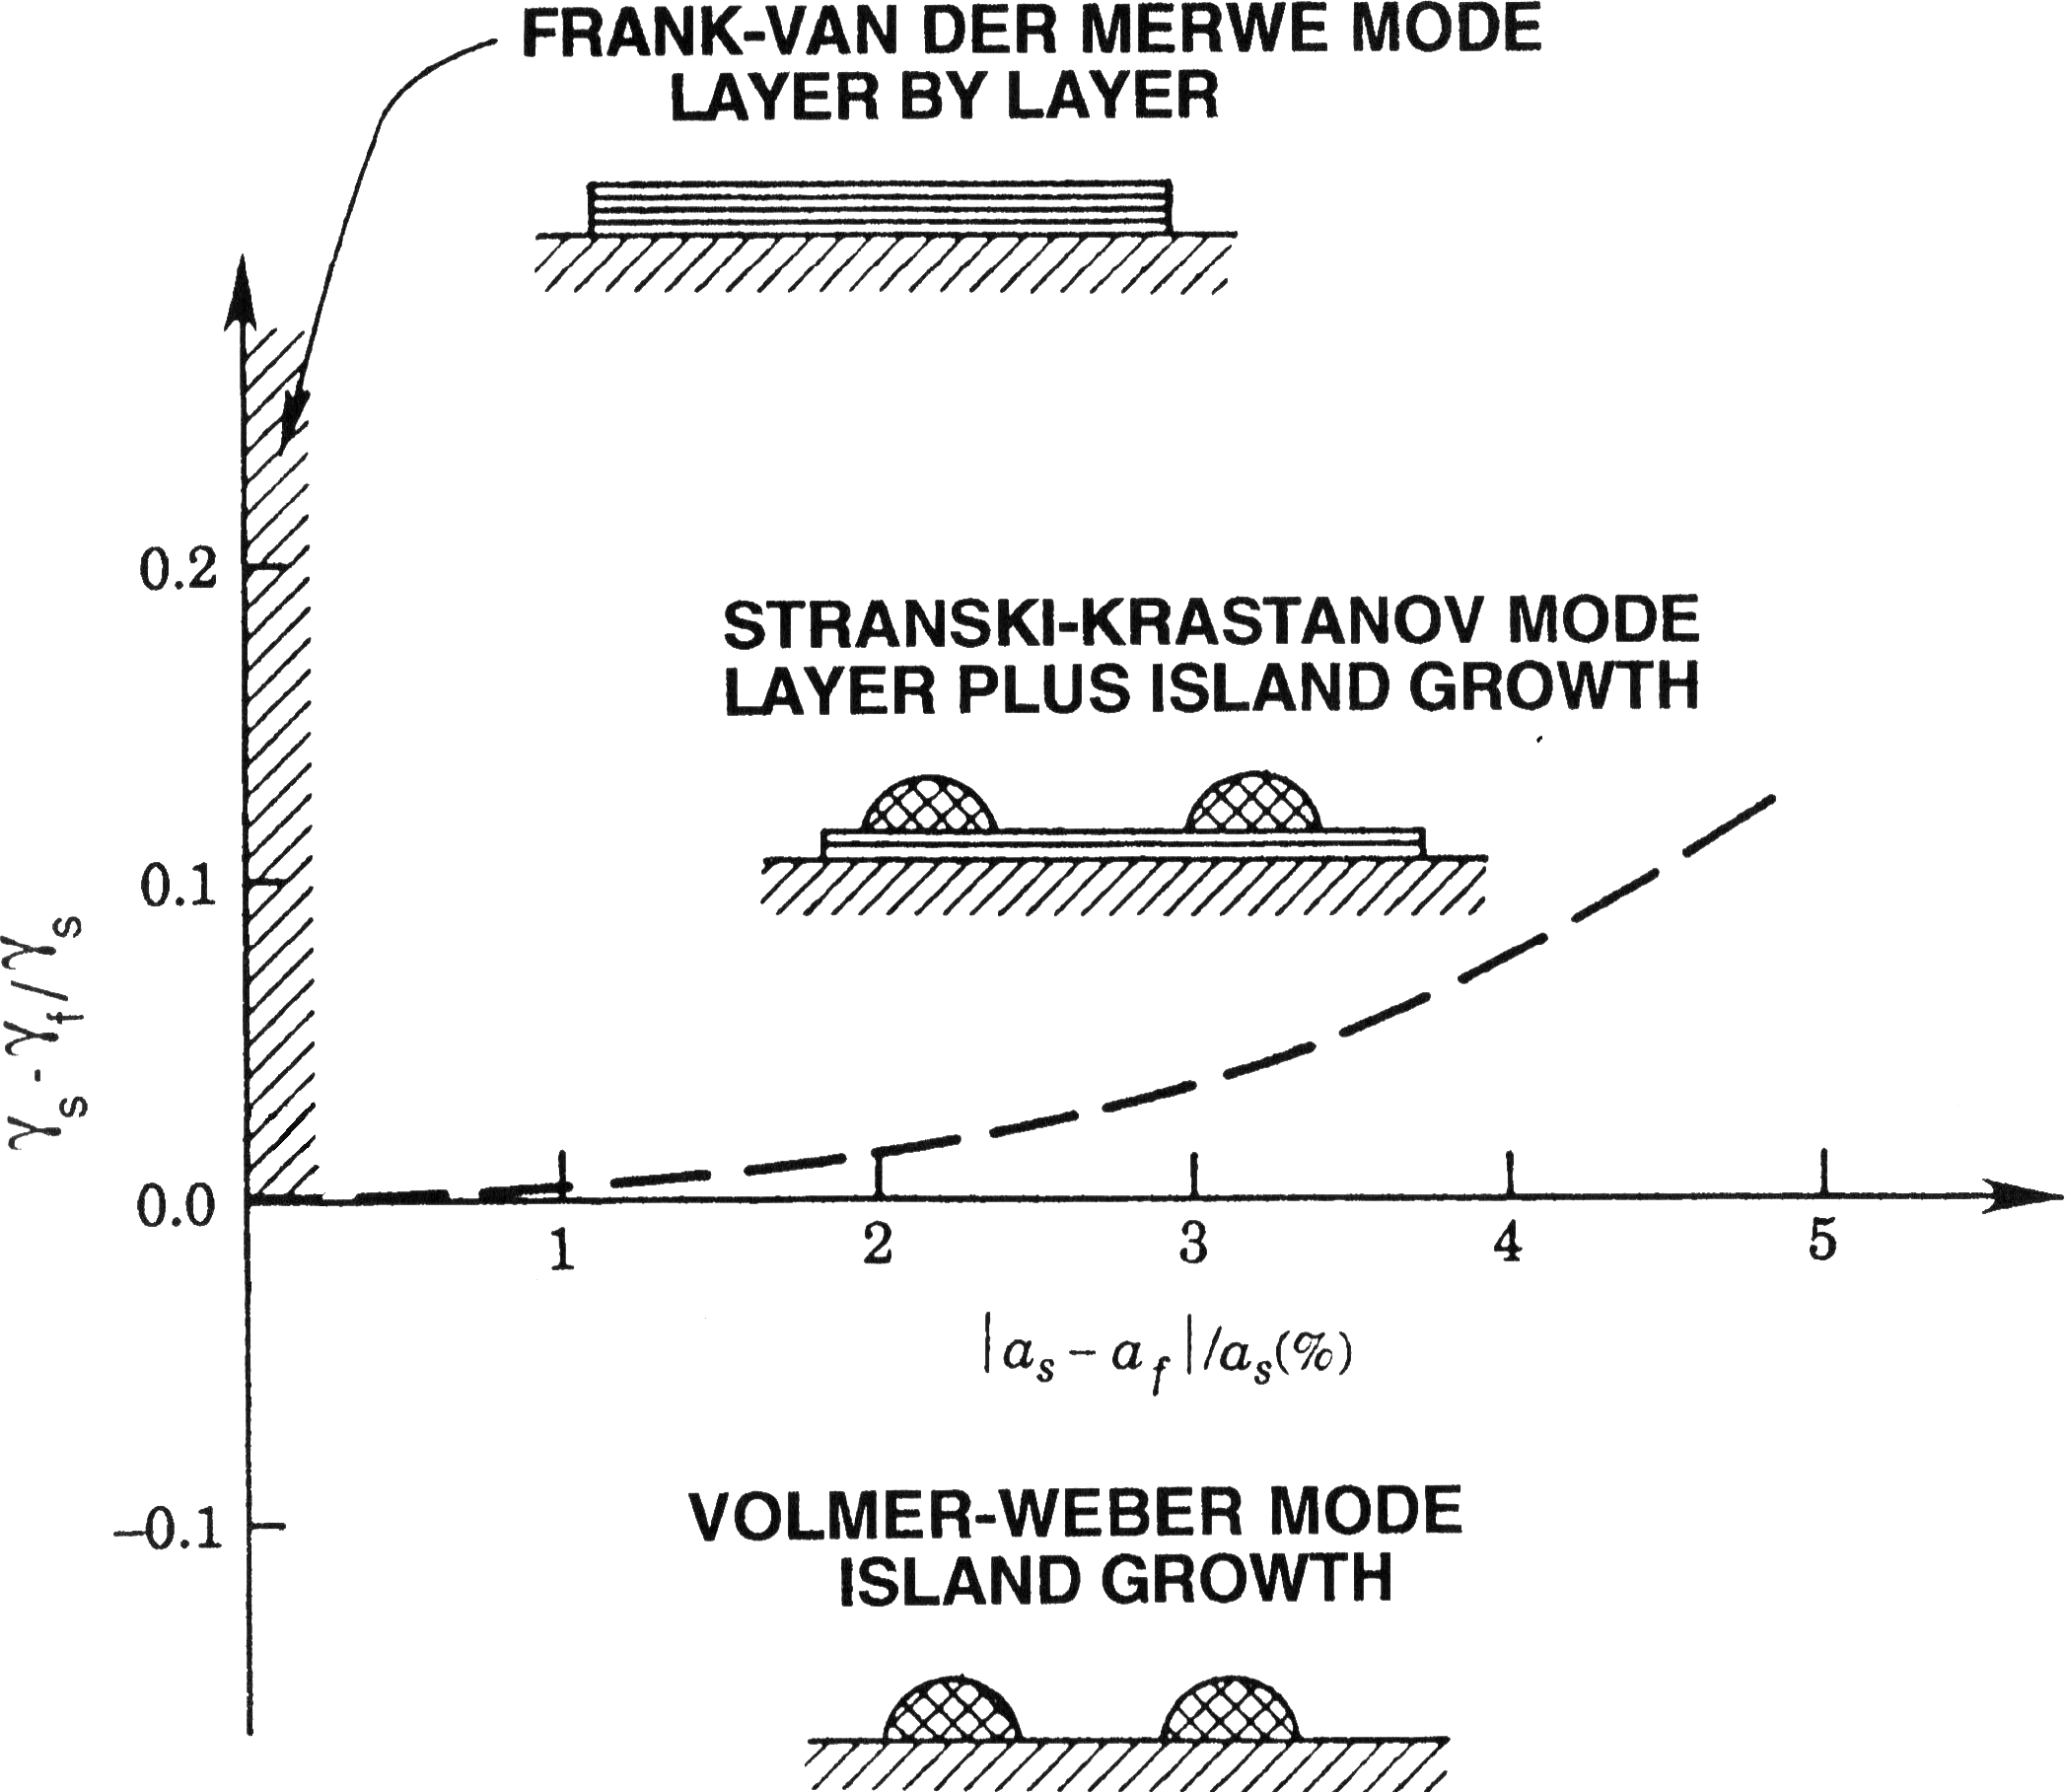
\includegraphics[width=0.8\textwidth]{back_nucleation_regions}
 \caption[Nucleation phase diagram of surface energy and strain]{\label{fig:back_nucleation_regions}Phase diagram showing regions of different thin film nucleation modes, plotted with axes of lattice mismatch (strain) and ratio of surface energies (used with permission after \cite{ohring2001materials})}
\end{figure}

\section{Surface Reconstructions}\label{sec:reconstruction}
If one were to consider a crystal of infinite size, and then cut it along any direction, the resulting truncated crystal surface would have a very high energy surface.
Bonds will be unsatisfied, there is likely to be an unbalanced charge, and the surrounding environment for each surface atom will be different than when it was in the bulk.
This high energy condition is not the equilibrium state and must be resolved.
The resolution of this high energy state that results when surfaces of a single crystal are exposed is called the surface reconstruction.
While the name surface reconstruction implies changes to just the surface atoms, a surface reconstruction can extend a number of atomic layers into the crystal.
Thus, the changes that occur at the surface of a crystal can result in a very different interface than the bulk crystal for the purposes of epitaxy.

The atoms on the surface of a newly cleaved crystal have a number of options for resolving their high energy configuration.
The simplest of options for atoms in those high energy states to reduce their energy is to move, that is, to change it's position relative to other atoms.
These movements happen both the in-plane and out-of-plane directions.
Both atomic translations can cause additional shifts in the atomic layers below the surface.
Both in-plane and out-of-plane atomic movement breaks the bulk symmetry of the original crystal, resulting in a surface with lower symmetry.
In extreme cases, atoms can migrate and form islands or otherwise cause faceting on the surface in order to minimize energy\cite{Duke1996,oura2010surface}.
A schematic example of the simple atomic movement and relaxation for surface reconstructions as shown in \cref{fig:back_recon_move}.
\begin{figure}
 \centering 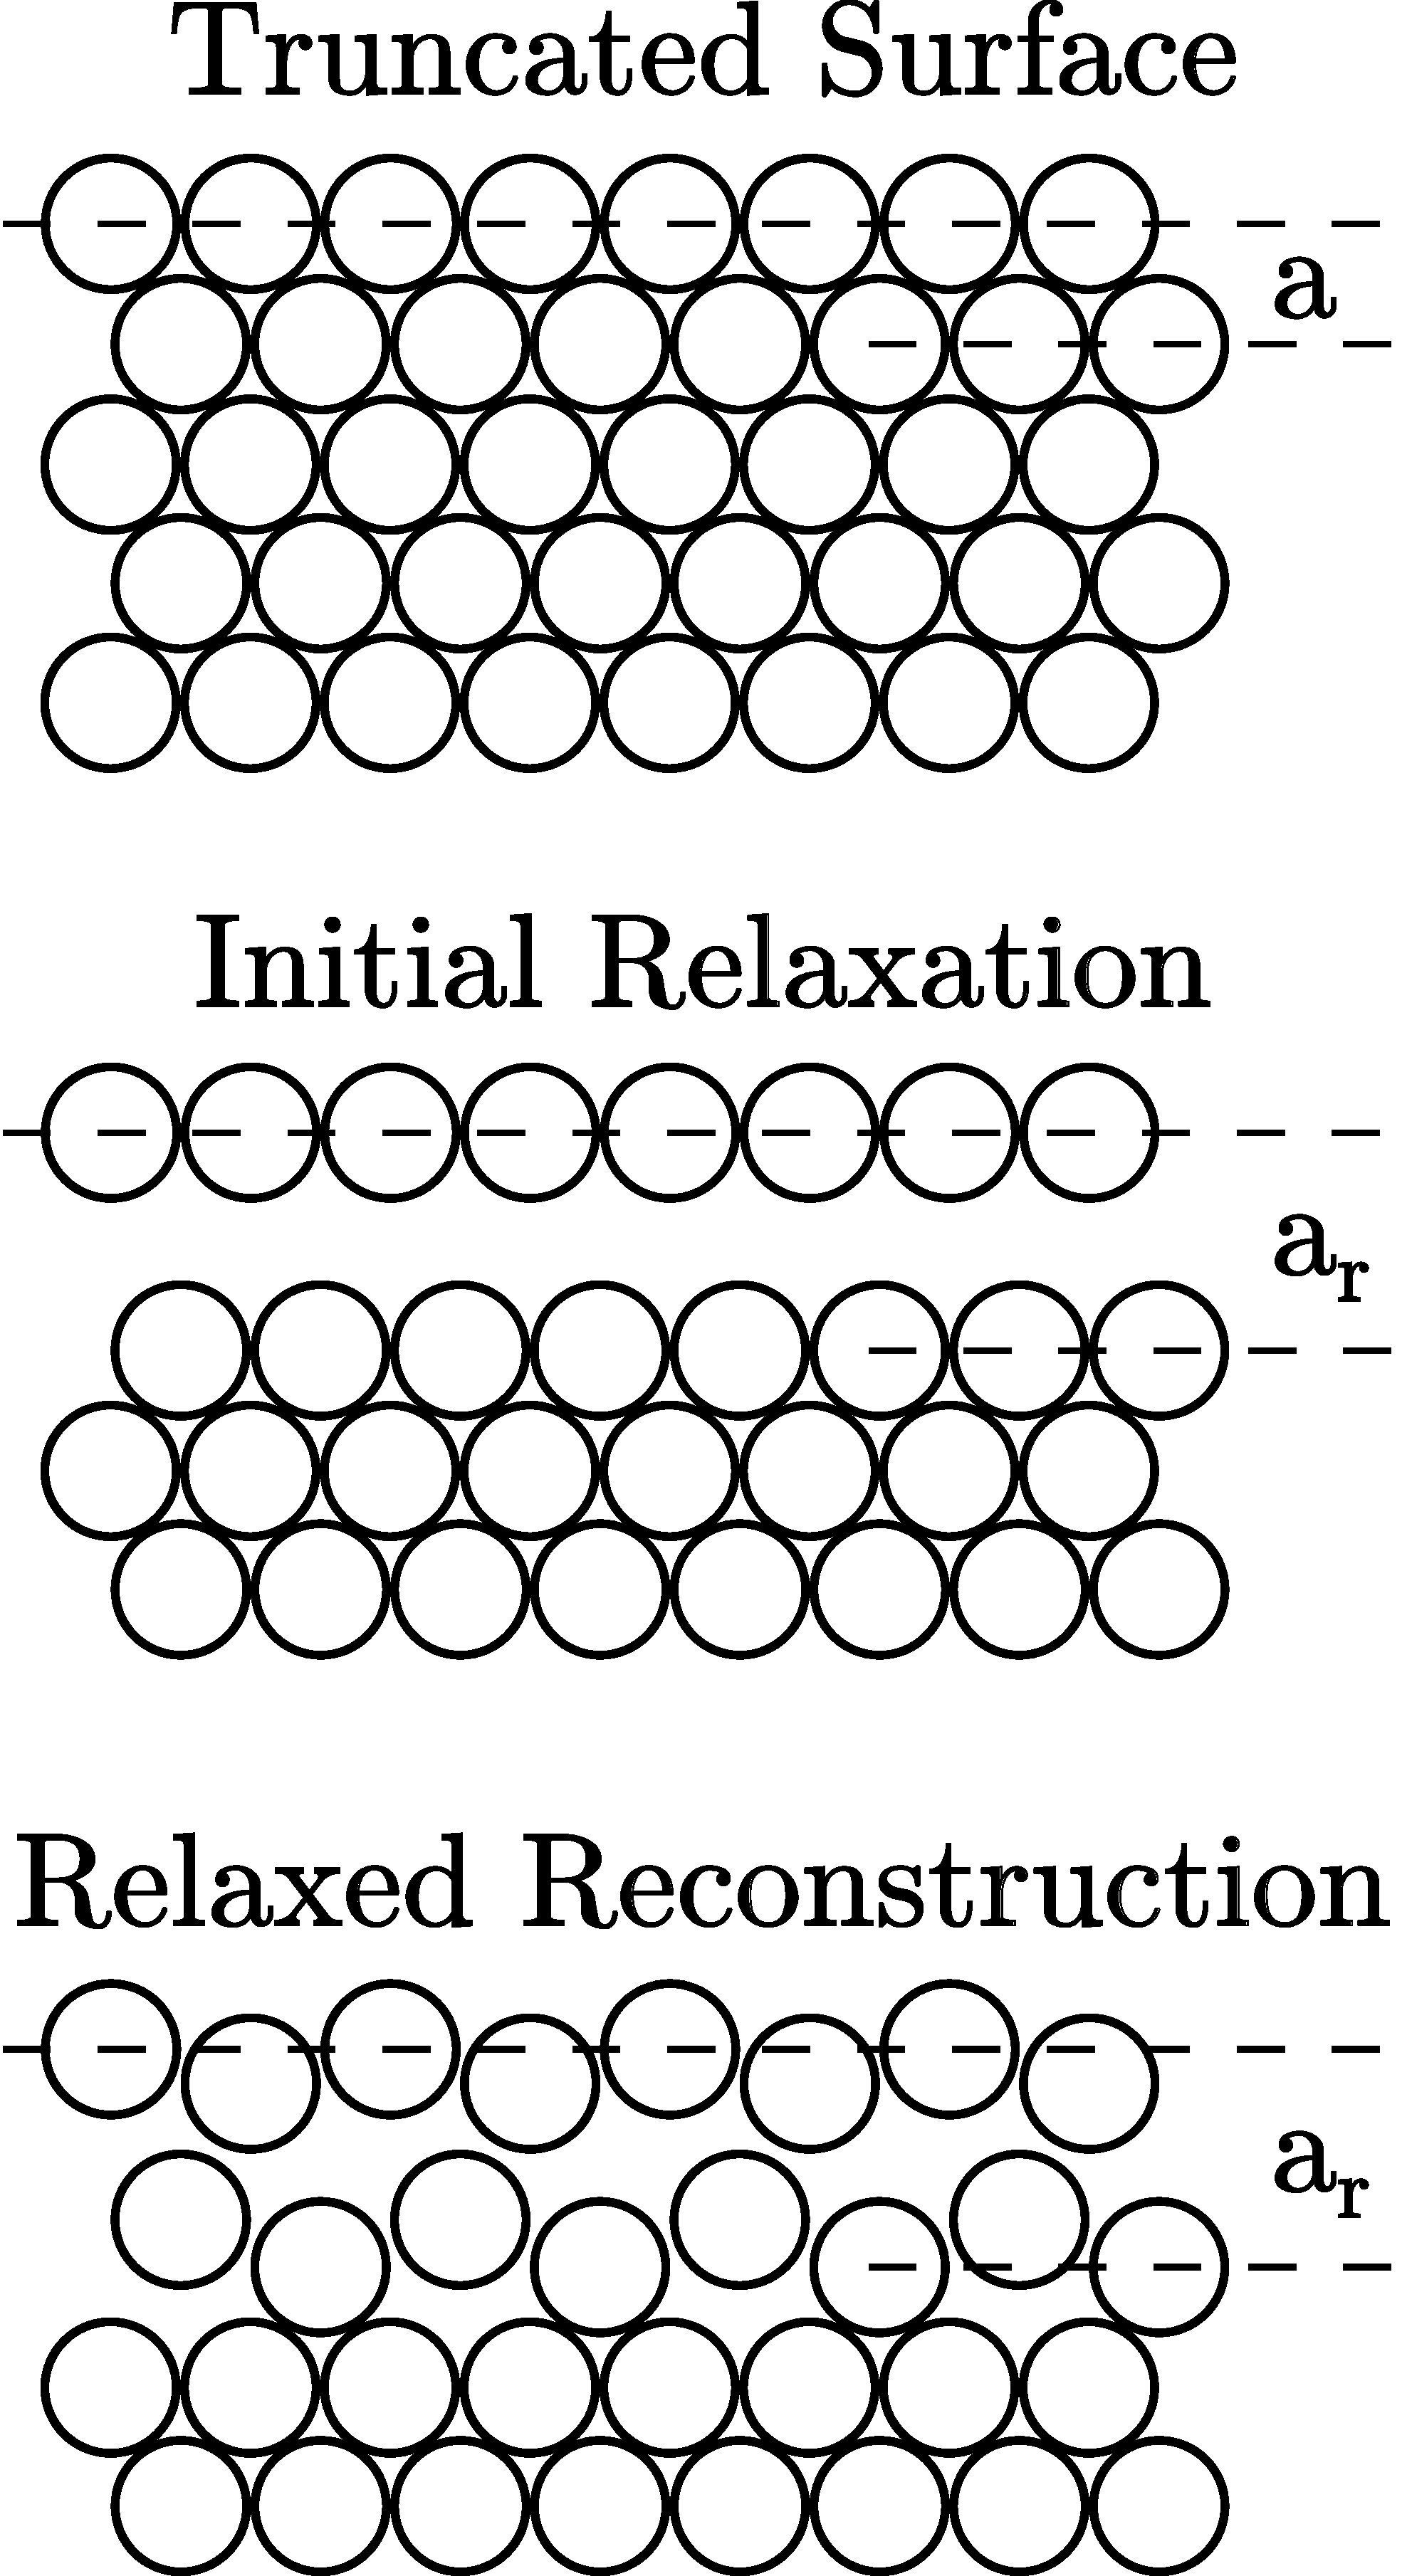
\includegraphics[width=0.5\textwidth]{back_recon_move}
 \caption[Simple surface reconstruction]{\label{fig:back_recon_move}The process of surface reconstruction with atomic movement a) truncated crystal b) layer movement due to no overlayer c) atomic roughening of surface to reduce total energy, with a\textsubscript{r} labelled as the reconstructed perpendicular lattice spacing (after \cite{ohring2001materials})}
\end{figure}

A more complex response resulting in a surface reconstruction that can arise is a change in the bonding in the upper layers of the crystal.
Dimers and higher order bonding can form at the surface of the crystal, partially resolving the dangling bonds present on the surface.
This dimerization of the surface can reduce the chemical activity of the surface since the electronic structure has been satisfied internally to the crystal\cite{Duke1996}.
One common example of the dimerization is that of the silicon (100) surface, as shown in \cref{fig:back_recon_dimer}.
\begin{figure}
 \centering 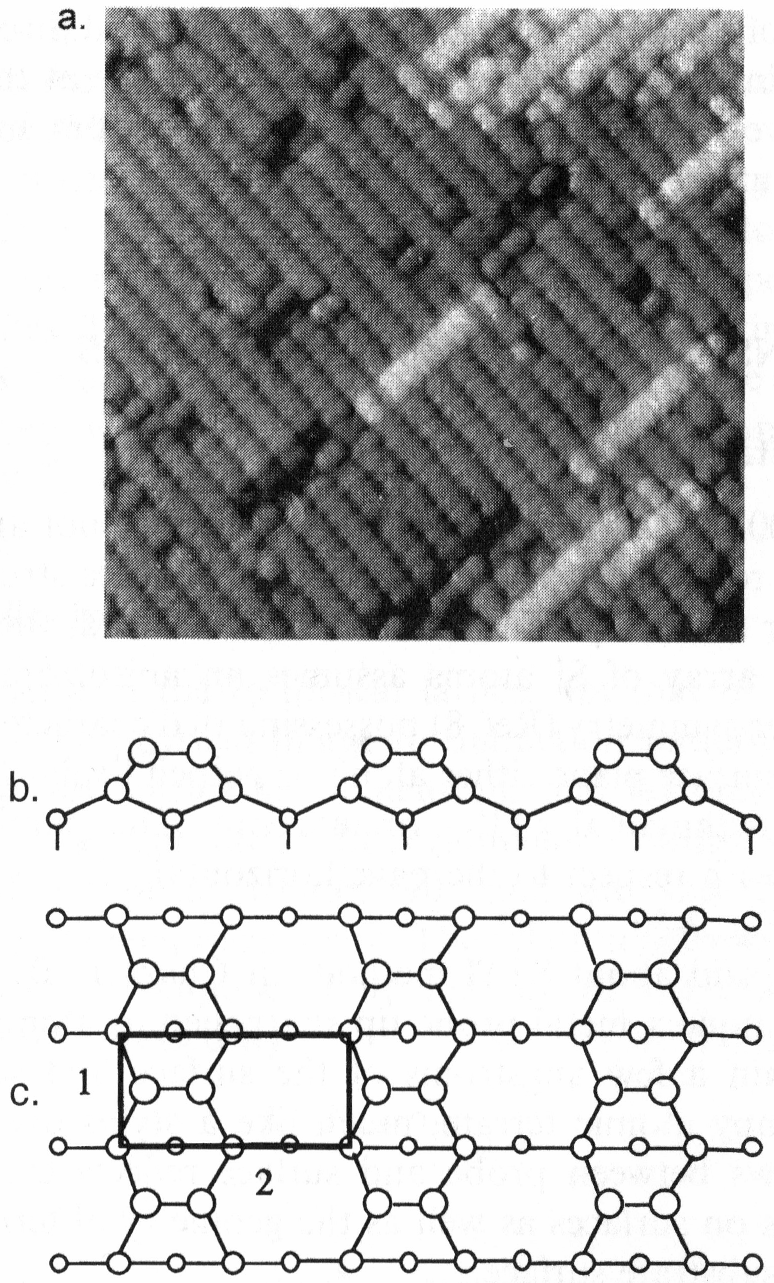
\includegraphics[width=0.7\textwidth]{back_recon_dimer}
 \caption[Silicon dimer surface reconstruction]{\label{fig:back_recon_dimer}a) STM of silicon surface reconstruction showing Si dimers b) cross sectional view of model (\(2 \times 1\)) surface reconstruction c) top view showing reconstructed surface unit cell after \cite{Zhang1997,Lagally1993}(used with permission)}
\end{figure}

Finally, a surface can reconstruct by ejecting some of the atoms which originally formed the surface.
The removal of such atoms can allow which was once a close-packed surface to have less density than the parent crystal lattice.
This is typical in reconstructions of materials where gaseous materials integrated into the lattice.
The resulting reconstruction can be multiple layers thick, progressively containing less atoms from the bulk to the surface.
Similarly, if reconstructions are formed in the appropriate atmosphere, the reconstruction can integrate additional atoms into the reconstruction.

\subsection{Cuts Along High-index Planes} When crystals are cut along low index planes (for example \{100\}, \{111\}, \{110\}  in cubic structures), surface reconstructions happen directly on these surfaces.
When crystals are cut along high index planes, there is additional energy associated with exposing non-close-packed planes.
These high index planes are highly unfavourable and do not have stable reconstructions.
The high index surface instead undergoes a breakup into sections of low index planes, separated by steps of fractional or multiples of the unit cell, as shown in \cref{fig:back_recon_vicinal}.
These low index planes can then further reconstruct as previously discussed.
\begin{figure}
 \centering 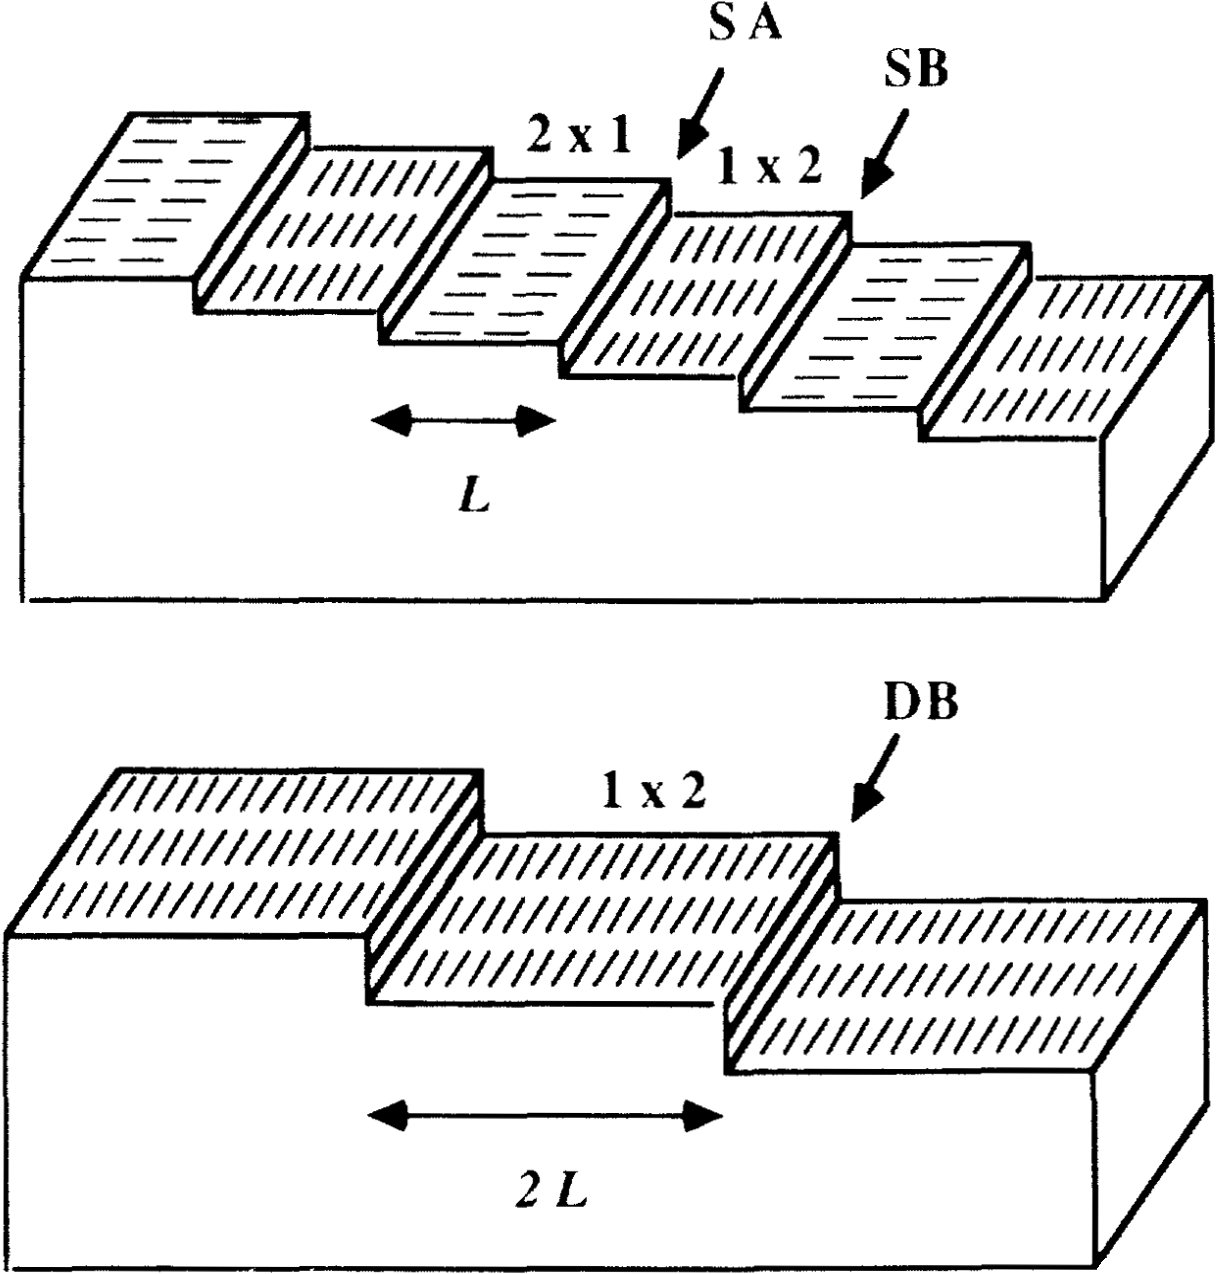
\includegraphics{back_recon_vicinal}
 \caption[Silicon single and double step surface reconstructions]{\label{fig:back_recon_vicinal}Vicinal silicon (100) surface reconstructions, a) single steps with alternating sublattices and dimers and b) double steps with the same sublattice exposed\cite{Alerhand1990}(used with permission, Copyright (1990) by The American Physical Society)}
\end{figure}

The most common case of high index planes exposed for surface reconstruction is offcut or vicinal surfaces.
The surfaces of single crystal wafers, when cut from a boule have a misalignment from the intended low-index plane due to processing error.
These wafers, when reconstructed form terraces of the low index plane, separated by fractional unit cell steps.
Steps are formed either as ``single'' (height \(\frac{a}{2}\)) or ``double'' (height \(a\)), with terrace lengths determined by the offcut angle, as in \cref{fig:back_recon_terrace} and \cref{eqn:back_recon_terrace}.
\begin{figure}
 \centering 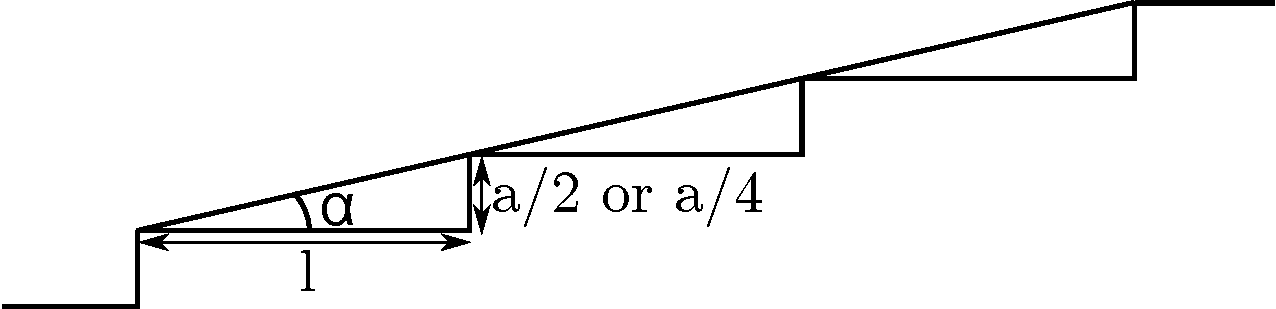
\includegraphics{back_recon_terrace}
 \caption{\label{fig:back_recon_terrace}Terrace length of reconstructed stepped surface due to offcut of \textalpha}
\end{figure}
\begin{equation}
 l = \frac{a}{\tan{\alpha}} \text{ or } l = \frac{a/2}{\tan{\alpha}} \label{eqn:back_recon_terrace}
\end{equation}

\subsection{Thermodynamics, Kinetics and Stability of Surface Reconstructions} While an unreconstructed crystal surface is in a high energy state, all the routes to lower energy states require an input of energy.
Thus, while a crystal surface may be in a high energy state after cutting, cleaving, polishing or other processing which exposes that surface, it can do very little to resolve its situation without help.
Energy must be inputted into the system to allow the atoms to move, bond or leave the surface.
The energy landscape of surface reconstructions has many local minima, so there are many possible surface reconstructions for a given surface, depending upon how much activation energy is provided to the system.
Beyond how much energy is delivered to the crystal, it takes time for the atoms to reach a one of local minima for the surface.
Some surface reconstructions can take a significant time to progress to completion, adding more energy in an attempt to speed up such reconstructions can result in transitions into another reconstruction, as such, time spent reconstructing is a key factor in the conditions of the final surface.

Thus far, energy and time have only been discussed in general terms.
The most successful and commonly used method of delivering energy and eliciting a reconstruction is to increase the temperature of the crystal.
Crystals can be annealed at a carefully controlled temperature for any desired amount of time.
Careful experimentation with annealing of crystals has resulted in ``phase diagrams'' of surface reconstructions given a surface and temperature combination, as seen in \cref{fig:back_recon_phase}.
\begin{figure}
 \centering 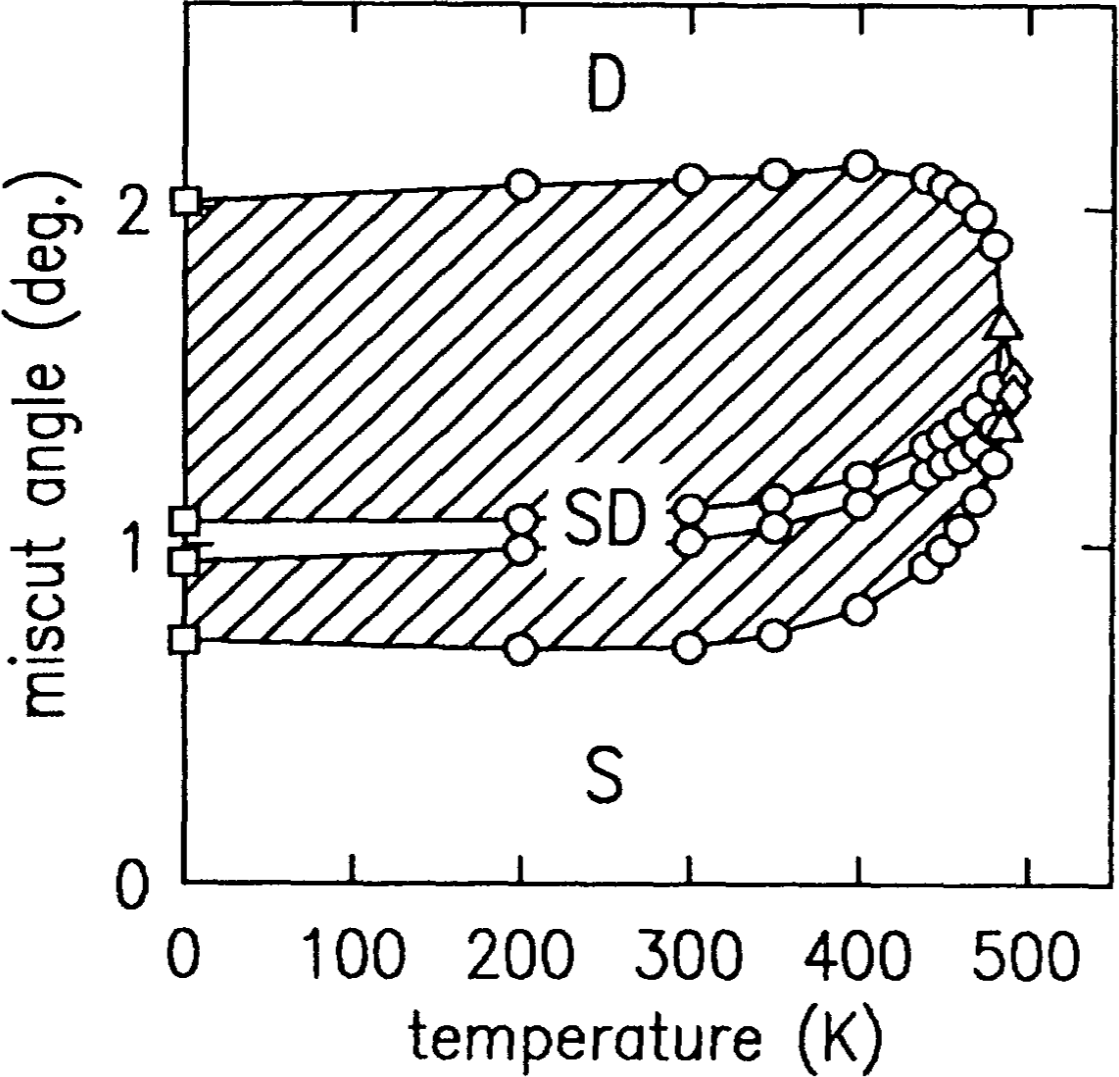
\includegraphics[width=0.6\textwidth]{back_recon_phase}
 \caption[Silicon surface reconstruction phase diagram]{\label{fig:back_recon_phase}Phase diagram of the Silicon (100) surface reconstruction showing regions of single and double steps, with shaded region of mixed reconstruction\cite{Pehlke1991}(Copyright (1991) by The American Physical Society)}
\end{figure}

The formation and stability of a given surface reconstruction also depends upon the environment surrounding the crystal.
Assuming the surrounding environment does not chemically react with a given crystal, the presence or absence (vacuum) of an inert gas will affect the activation energies for the surface atom processes.
A vacuum above a crystal when annealing promotes the exit of atoms from the surface as there is force resisting the atoms, or back scattering them towards the surface.
For complex crystals which incorporate elemental gasses into their lattice, different surface reconstructions are achievable if an overpressure of those gasses are present, rather than a vacuum.
These surface reconstructions are commonly seen in the complex oxides, where oxygen is a primary constituent of the crystal and will be lost from the surface during annealing if an overpressure is not provided.

Stability of surface reconstructions to subsequent interactions with atoms added to the surface varies widely depending upon the properties of the crystal.
Semiconductor crystals have less stable surface reconstructions, interactions with additional atoms easily destroy an established reconstruction.
The most common example are the common silicon reconstructions, which are disrupted and destroyed during epitaxy of additional layers.
Refractory crystals (defined as those materials high melting points and with stability above 538\celsius{}\cite{ASTMC71}, such as MgO T\(_m\) = 2852\celsius{}, Al\(_2\)O\(_3\) T\(_m\) = 2072\celsius{} and MgAl\(_2\)O\(_4\) T\(_m\) = 2130\celsius{}) such as complex oxides are considerably more stable once reconstructed, a point which has been taken advantage of later in this work.

\subsection{Nomenclature for Surface Reconstructions} Since surface reconstructions are pseudo-2D constructs, the allowed symmetries of a surface reconstruction are a subset of those of the allowable 3D lattices.
There are five unique 2D surface nets that can be used to describe the symmetry of a surface reconstruction as shown in \cref{fig:back_recon_lattices}
\begin{figure}
 \centering 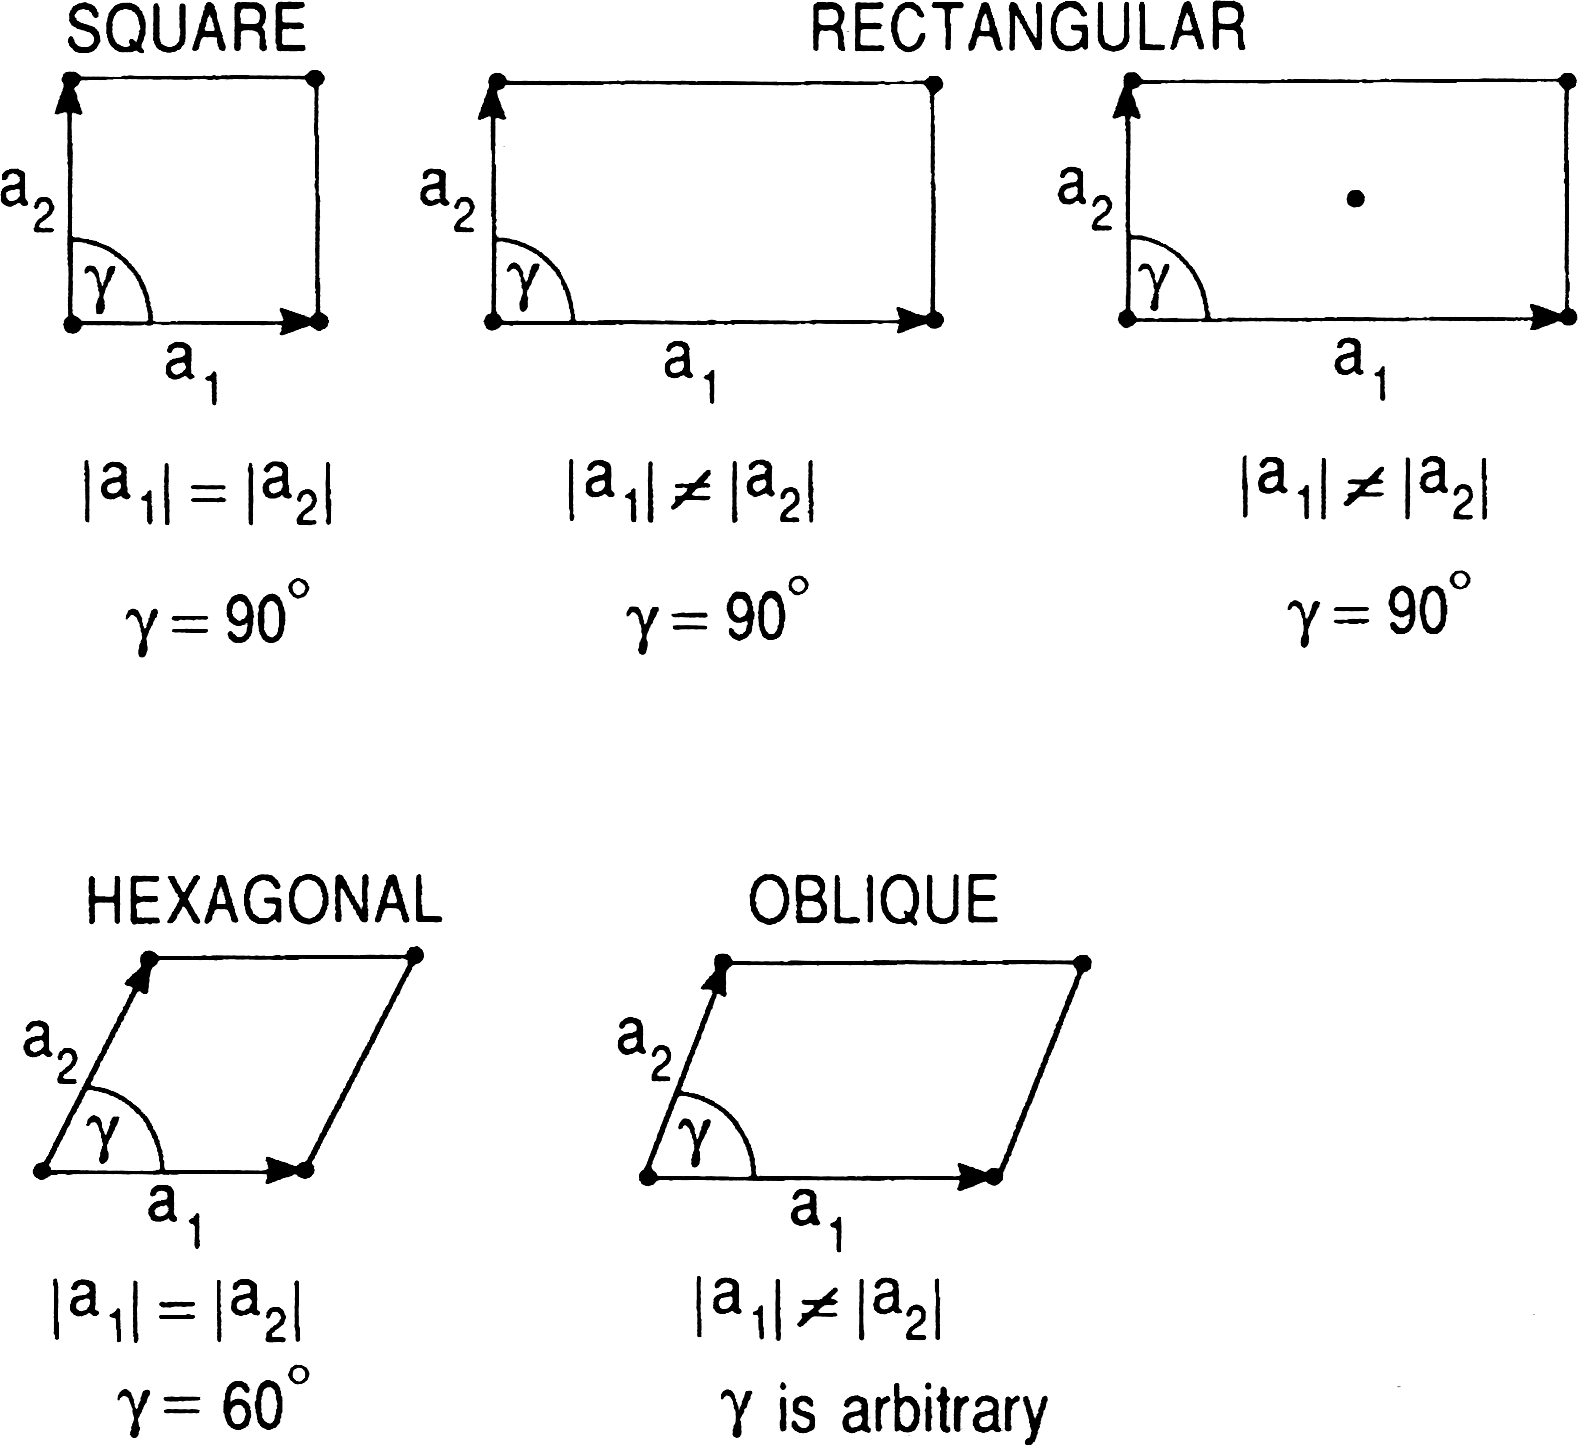
\includegraphics[width=0.8\textwidth]{back_recon_lattices}
 \caption[2D Surface Nets]{\label{fig:back_recon_lattices}The five unique 2D surface nets, all are primitive (single atom basis) except for the two atom centred rectangular net (after \cite{ohring2001materials})}
\end{figure}

The nomenclature of naming surface reconstructions is determined by the relationship of the 2D surface lattice to the underlying unit cell.
The notation preferred in the literature was originally introduced by Wood\cite{Wood1964} The smallest repeating surface cell is determined and denoted by whether it is primitive (\textbf{P}), having only one atom per surface cell, or centred (\textbf{C}).
The surface cell's repeat unit is then related to underlying unit cell by the ratio of the surface cell lattice constant to the unit cell lattice constant.
Thus, the simplest surface reconstruction for a crystal would be the P(\(1 \times 1\)) reconstruction, containing one atom, and having the same spacing as then underlying crystal.
These nomenclatures do not include details such as the type, number or configuration of atoms which constitute the reconstruction.
These reconstructions can also be rotated relative to the underlying unit cell being denoted by \textbf{R}\@. A number of example surface reconstructions namings are shown in \cref{fig:back_recon_name_examples}.
The nomenclature for surface reconstructions is not unique, as a reconstruction such as C(\(2\times2\)) is equivalent to
(\(\sqrt{2}\times\sqrt{2}\))R45\degree{}
reconstruction.
\begin{figure}
 \centering\ 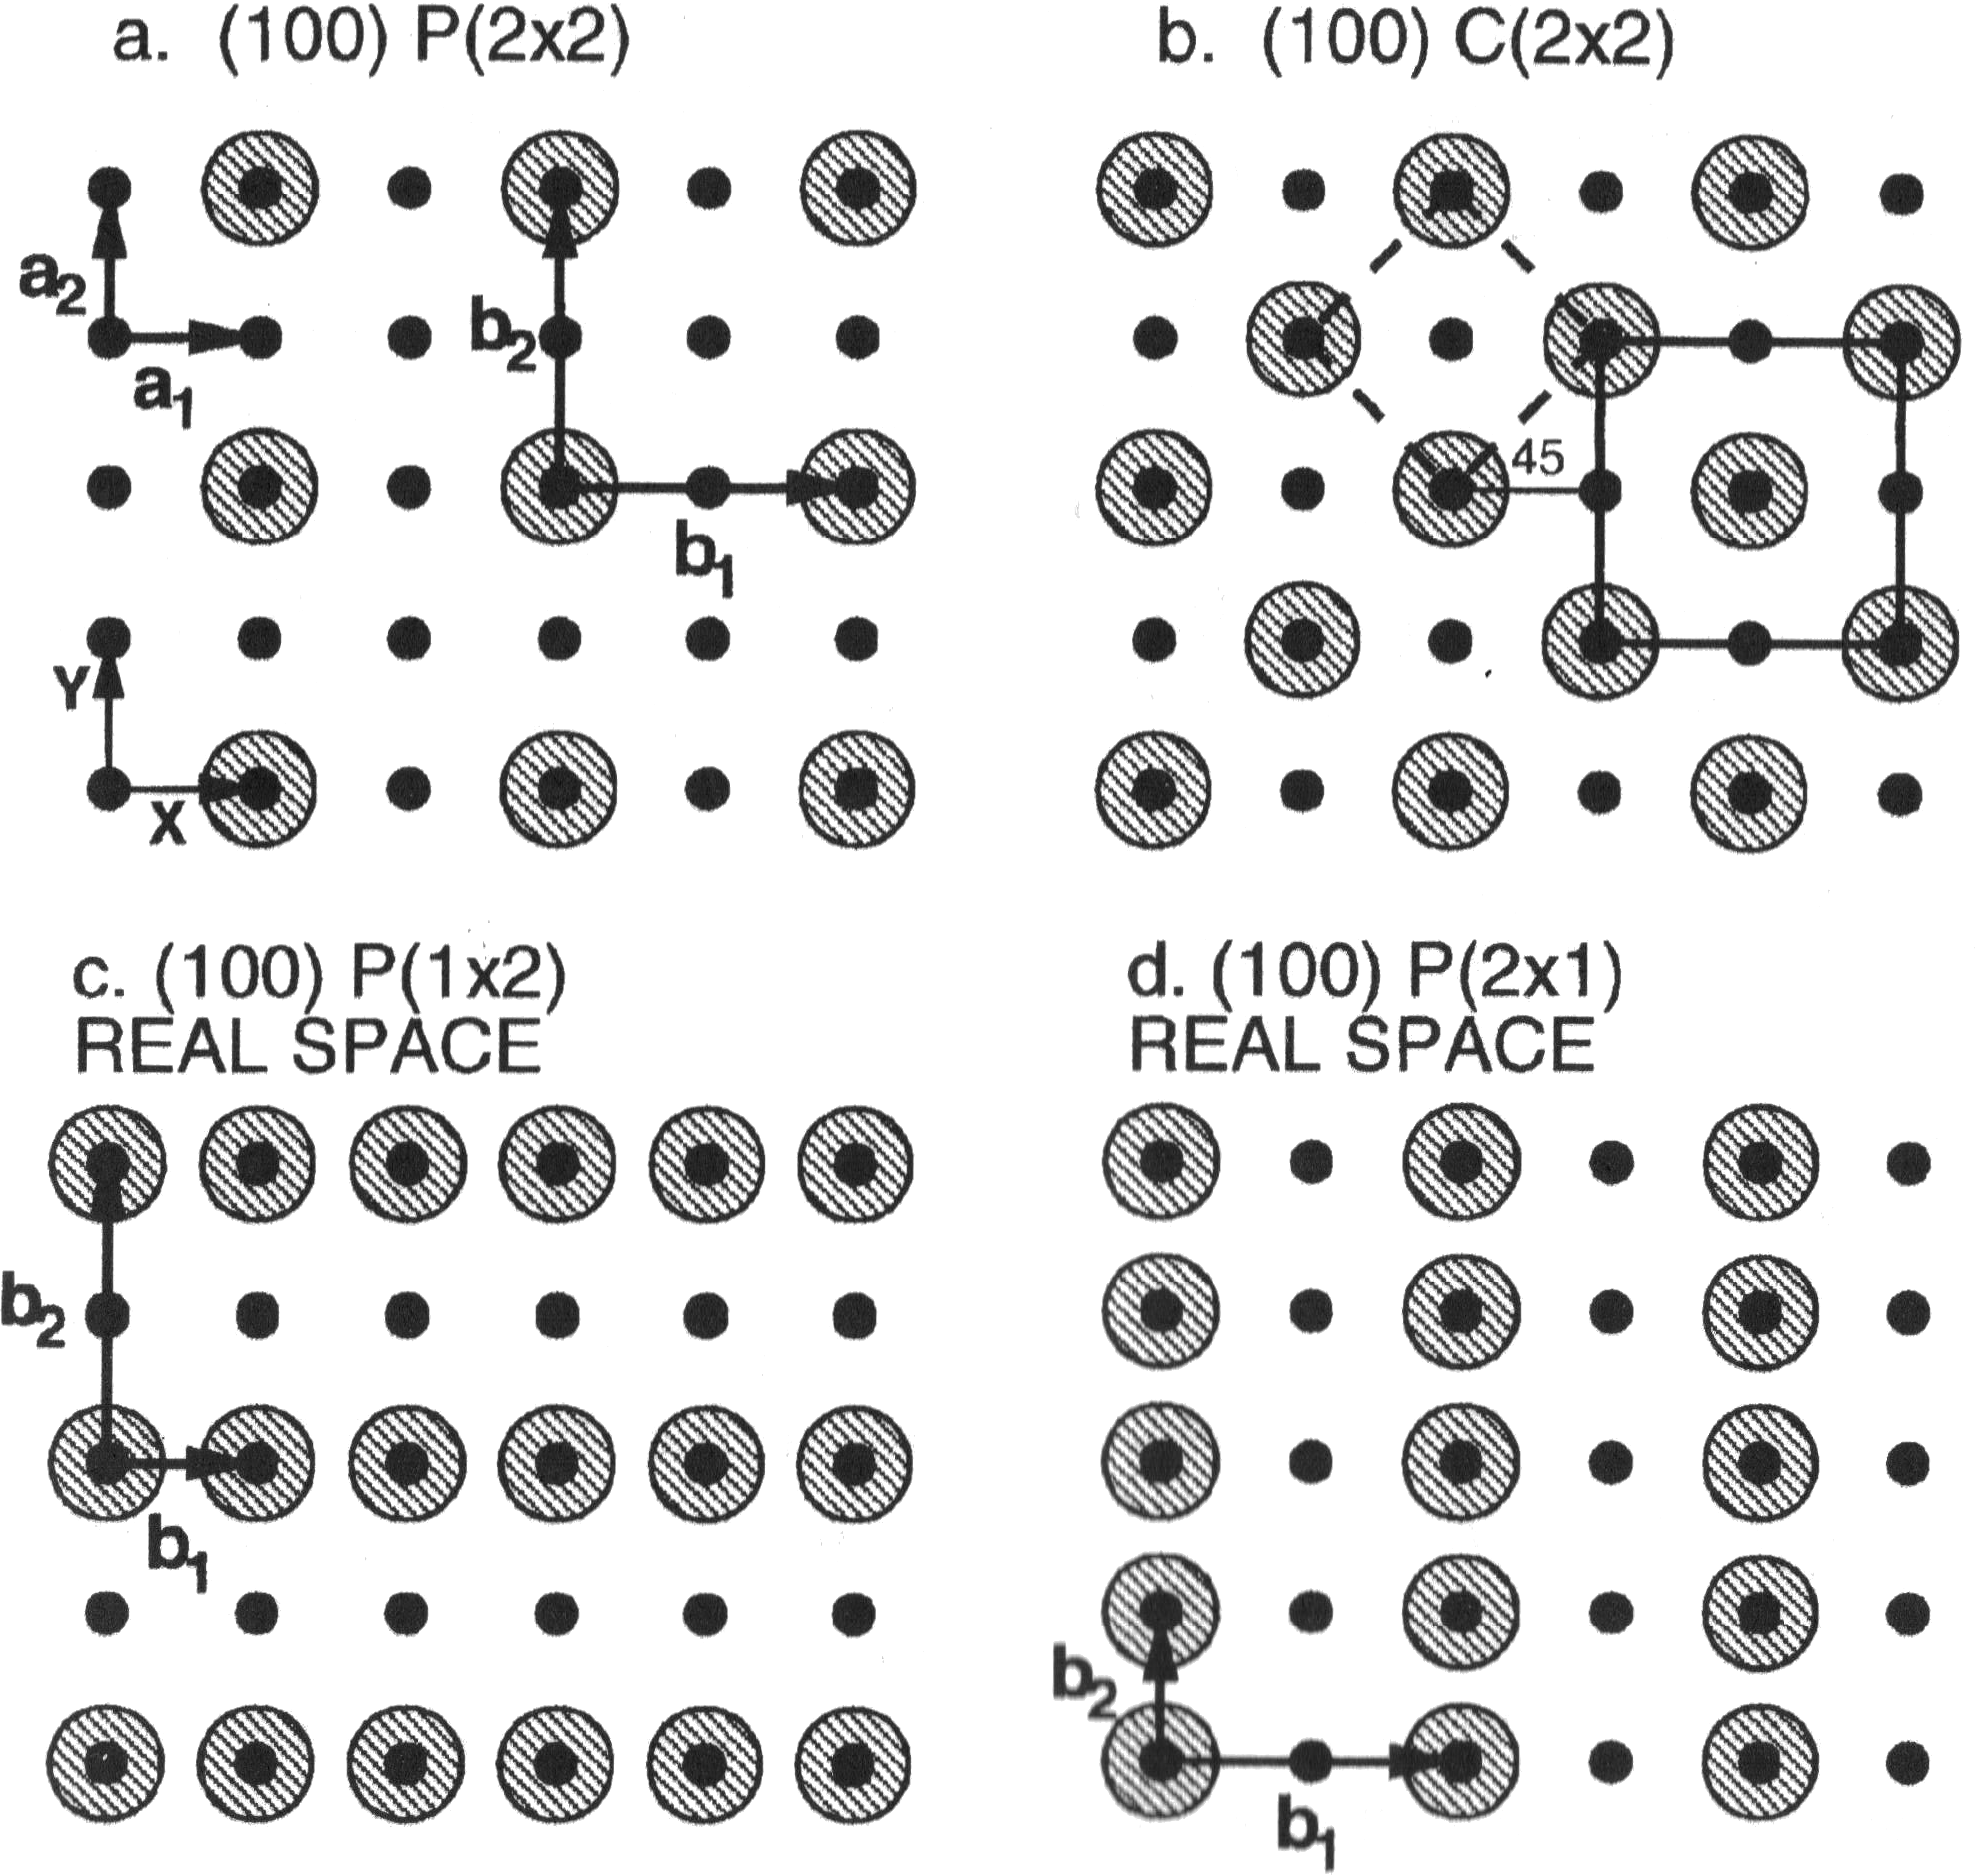
\includegraphics[width=0.9\textwidth]{back_recon_name_examples}
 \caption[Examples of surface reconstructions]{\label{fig:back_recon_name_examples}Examples of simple cubic surface reconstructions showing atomic positions of reconstructed atoms (shaded) relative to bulk atoms (dots) on a (100) simple cubic substrate.
  a) P(\(2 \times 2\)) b) C(\(2 \times 2\)) or
  (\(\sqrt{2}\times\sqrt{2}\))R45\degree{}
  c) P(\(1 \times 2\)) d) P(\(2 \times 1\)) (used with permission after \cite{ohring2001materials})}
\end{figure}

\section{Atomic Bonding --- Attraction Between Atoms}
The strength of attraction between atoms is a key factor in the growth process of epitaxial crystals.
Attraction between atoms in a crystal is dominated by three different types of forces, electrostatic attraction, covalent electronic attraction and dipole attraction.

Electrostatic attraction is the major contributing force in ionic materials.
In such systems, atoms exchange electrons due to their large differences in electronegativity and the resulting anions and cations are bonded together via electrostatic attraction.
With multiple atoms, the anions and cations are alternately surrounded by cations and anions, allowing the formation of crystals.
A common example of purely electrostatic or ionic material is sodium chloride, where each sodium atom (Na) loses its electron to a chlorine atom (Cl) to form a repeating structure of Na\(^+\) and Cl\(^-\).

Covalent electronic attraction is the typical type of attraction seen in most molecules and many crystalline materials.
When atoms come together they change their electronic structure to hybridize and share their outermost electronic orbitals.
These shared orbitals lower the overall energy of the system, resulting in a strong bonding force between the two atoms.
These bonds, sometimes called chemisorption, typically have energies of 1--10~eV\cite{oura2010surface}.
When multiple atoms are brought together, they can hybridize and share atomic orbitals between more than one atom, allowing for a multitude of configurations and the diversity of crystal symmetries seen in nature.
An example of a purely covalent material is silicon, where each atom has hybridized its electronic orbitals and shares its orbitals equally with four surrounding silicon atoms.
\begin{figure}
 \centering 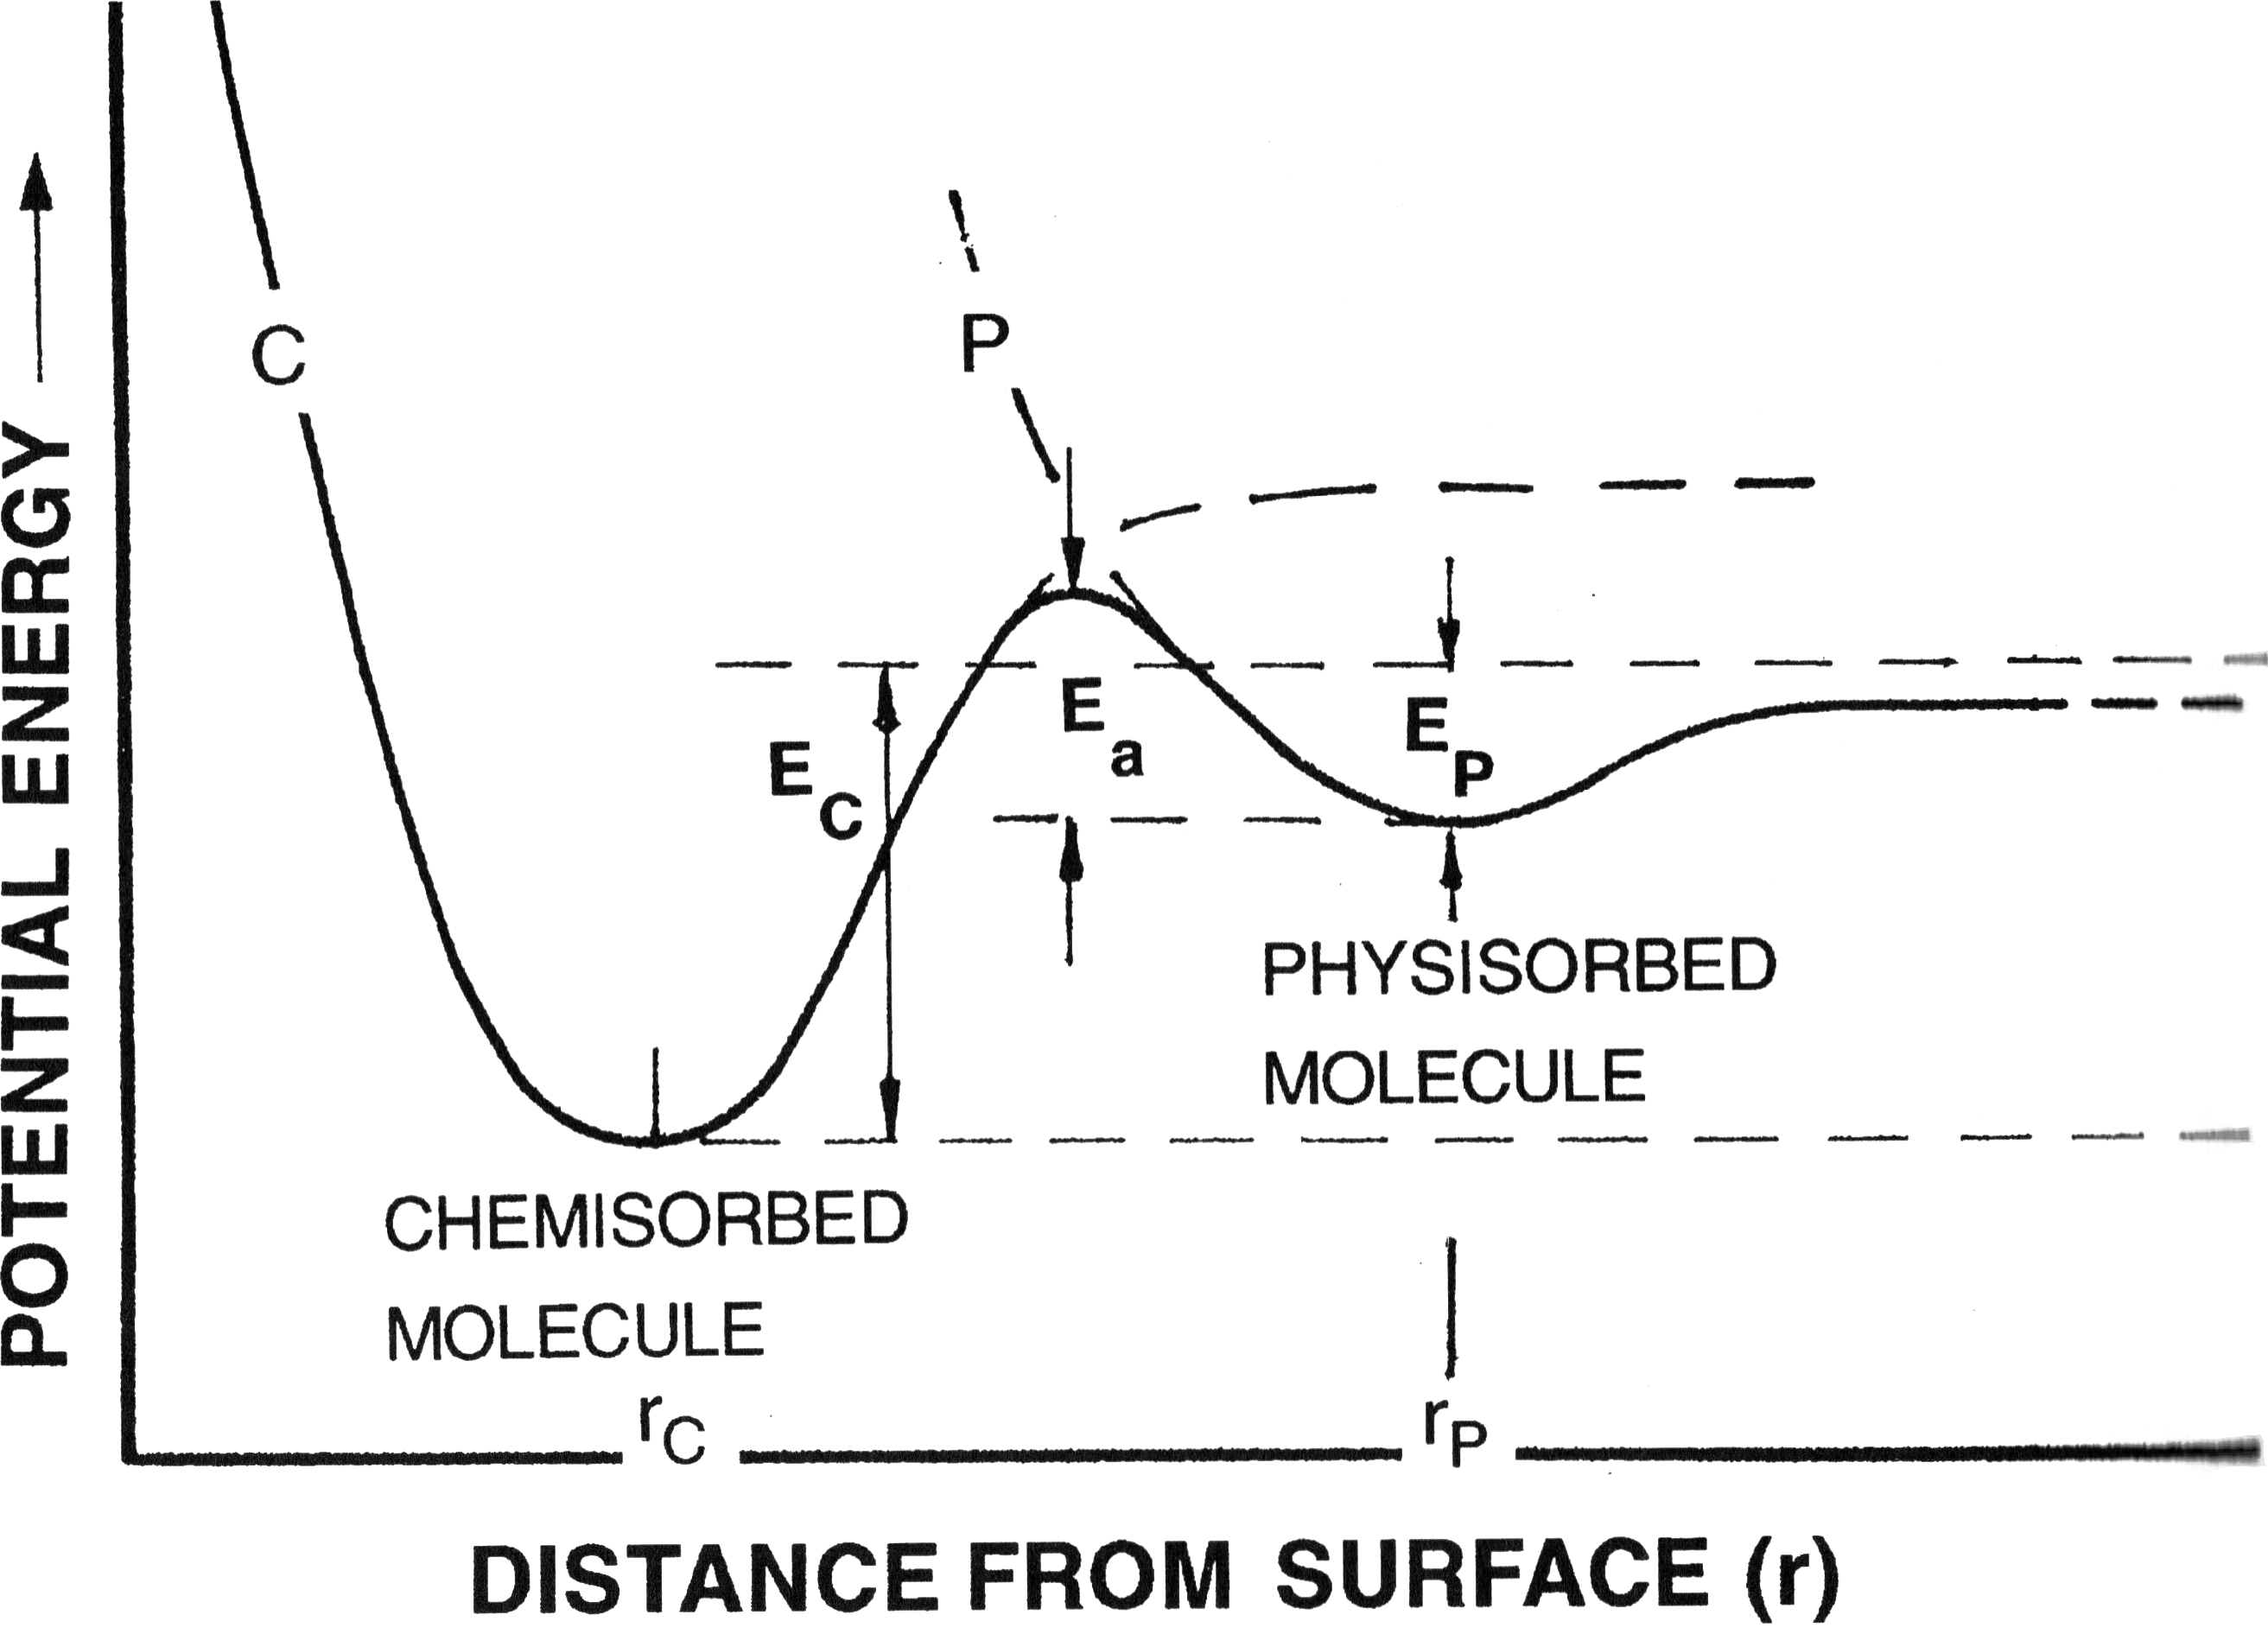
\includegraphics[width=0.6\textwidth]{back_bond_potential}
 \caption[Energy potentials between two atoms]{\label{fig:back_bond_potential}Potential energy versus distance for atom respect to surface, showing the region of adsorption and chemisorption\cite{ohring2001materials} (used with permission)}
\end{figure}

Hydrogen attraction is a type of atomic interaction potential which acts on the permanent dipoles formed in compounds with hydrogen.
While it is a substantial component of the properties of water it is rare in crystalline materials and needs no further consideration here.

Van der walls attraction is the third of the atomic interaction potentials.
Van der Walls attraction is due to the dipole-dipole interactions between the electronic structure of atoms.
Such an attraction process is different than covalent, the electronic structures are attracted due to their oscillating polarizabilty of the electron could, but do not share or hybridize electronic structures.
These atomic interactions occur at greater distances than covalent interactions, and are considerably weaker, generally having potentials of 10--100~meV\@. The Van der Walls potential is the force that initially binds adatoms at the epitaxial interface, sometimes denoted physisorption, allowing them to move freely on the surface before chemically reacting and becoming covalently bound.
The potential energy of an atom approaching a surface is shown qualitatively in \cref{fig:back_bond_potential}, showing the first energy minimum of physisorption and the second deeper potential energy minimum of chemisorption.

In real materials, the bonding is more complicated than the three distinct potentials described.
Many materials have both a covalent and an ionic nature at the same time, a property described as ionicity.
In such materials, the electronic orbitals for the atoms hybridize as with covalent systems, but the resulting shared orbitals are unequal.
Due to differences in electronegativity, one atom will contain a larger amount of the electronic charge, causing an electrostatic attraction between the atoms in addition to the covalent attraction.
Most materials fall into this category of having a partial ionic nature.

In addition to the partially ionic nature of some solid materials, other materials also contain a partial Van der Walls nature.
Generally, such materials consist of stacked layers of covalently bonded atoms which have their electronic orbitals fully satisfied.
These layers of atoms, by virtue of being atomically flat, come into close contact with adjacent layers, close enough that their electronic orbital dipole moments cause attraction, allowing for stable stacking.
A common example of such a material is graphite, an allotrope of carbon, in which the carbon atoms hybridize and covalent attract in a single atom thick layer, which are then attracted to each other via Van der Walls forces.
Such bonding is rare in epitaxial systems but may of relevance to the epitaxial liftoff phenomenon examined later.


